%%%%%%%%%%%%%%%%%%%% author.tex %%%%%%%%%%%%%%%%%%%%%%%%%%%%%%%%%%%
%
% sample root file for your "contribution" to a proceedings volume
%
% Use this file as a template for your own input.
%
%%%%%%%%%%%%%%%% Springer %%%%%%%%%%%%%%%%%%%%%%%%%%%%%%%%%%


\documentclass{svproc}
%
% RECOMMENDED %%%%%%%%%%%%%%%%%%%%%%%%%%%%%%%%%%%%%%%%%%%%%%%%%%%
%

% to typeset URLs, URIs, and DOIs
\usepackage{url}
\usepackage[utf8]{inputenc}
\usepackage{graphicx}
\def\UrlFont{\rmfamily}

\begin{document}
\mainmatter              % start of a contribution
%
\title{Person Following Robot Behavior Using Deep Learning}
%
%
\author{No author is given}
\author{Ignacio Condés\inst{1} \and José María Cañas\inst{2}}
% %
% %
\institute{Universidad Rey Juan Carlos,
 	\email{ignacio.condes.m@gmail.com},
 	\and
 Universidad Rey Juan Carlos, \email{jmplaza@gsyc.urjc.es}}

\maketitle              % typeset the title of the contribution

\begin{abstract}
Human-robot interaction (HRI) is a field with growing impact as robot applications are entering into homes, supermarkets and general human environments. Person following is an interesting capability in HRI. This paper presents a new system for a robust person following behavior inside a robot. Its perception module addresses the person detection on images using a pretrained TensorFlow SSD \emph{Convolutional Neural Network} which provides \emph{robustness} even on tough lighting conditions. It also includes a face detector and a \emph{FaceNet} CNN to reidentify the target person. Care has been put to allow real-time operation. 
%A \emph{person tracker filter} has been included to alleviate the effect of false positives/negatives. It also extracts faces, which are also analyzed by a \emph{FaceNet} CNN to reidentify the tracked individual. 
%This perception module tells which person in the image has to be followed, even on poorly lightened scenarios. 
%It is combined with depth readings to obtain the relative position of the person. 
The control module implements two \emph{PID} controllers for a reactive smooth response, moving the robot towards the target person without distracting with other people around. The entire system has been experimentally validated on a real TurtleBot2 robot, with an Asus Xtion RGBD camera.
% We would like to encourage you to list your keywords within
% the abstract section using the \keywords{...} command.
\keywords{Computer Vision, neural networks, deep learning, robotic behavior}
\end{abstract}
%

%  ---- Intro ----
\section{Introduction}
%
In this project, we aim to establish a scope which covers two fields: \emph{robotics} and \emph{deep learning}.\\

In the last decades, robots have become a powerful allied to humans, as they are leveraged to perform all kind of tasks (hazardous explorations, personal assistance, cleaning, driving, \dots). However, we aim to design them to perform these tasks on the most autonomous way possible, which means not requiring to be controlled on every action (with exceptions, such as surgeon robots). This requires to provide robots a certain intelligence and capabilities to correctly trigger the most suitable action for each possible input stimulus. For this purpose, we can find multiple approaches for different problems (navigation, conversation, \dots).\\

Concretely, this article is dovetailed with \emph{Computer Vision}, which involves connecting cameras to a robot, and taking advantage of this on an autonomous way. Concretely, we will tackle the \emph{person following} challenge, which is based on a behavior governed by a person \emph{detection} system. Many approaches are already existing, such as color filters \cite{rocapal}, or disparities filtering. However, promising \emph{Deep Learning} techniques excel on their image processing variant, as they offer high quality results, accompanied by \emph{robustness} facing lighting issues (Fig. \ref{fig:intro_harsh_light}). This is the set of techniques we have used on this project, so we will describe the basis firstly.\\

\begin{figure}[h]
	\centering
	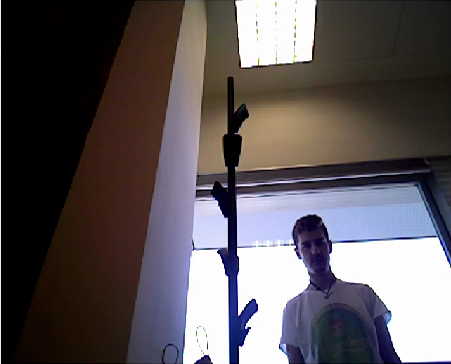
\includegraphics[width=2in]{images/light_ko_2}
	\caption{Harsh lighting situation for \emph{Computer Vision} algorithms.}
	\label{fig:intro_harsh_light}
\end{figure}


In the image detection quandary, the main objective is to determine \emph{presence and position} of a certain object in a given image. For this, we make use on this article of \emph{deep learning} techniques, concretely \emph{Convolutional Neural Networks} (CNNs).\\


This investigation has focused on exploring the synergies existing the two explained fields, making use of \emph{deep learning} to automatically command a robot to follow a determined person. This is achieved making use of two different modules: a \emph{perception} one, focused on the computer vision/deep learning tasks, and an \emph{actuation} module, which implements a case-based behavior, depending on what the perceptive part senses and computes. The designed system has been experimentally validated, as it will be seen on section \ref{sec:experiments}

% ---- State of the art ----
\section{Related works}

The person following behavior is a old problem in Human-Robot-Interaction field with many existing solutions in the literature \cite{sidenbladh1999person,rocapal2005,yoshimi2006development}. 

%Human detection 
A nice approach \cite{aguirre2016multisensor} uses laser sensors to detect the legs, sensor fusion and a particle filter to provide robustness and continuity to the person estimation. 

The topic has been extensively explored using a single camera \cite{yoshimi2006development}. Other interesting approaches use stereo vision. \cite{munoz2007people} combines color of the clothes and position information to detect and track multiple people around. They use Kalman filters and fuse the plain-view map information with a face detector. \cite{satake2009robust} use depth templates of person shape applied to a dense depth image and an SVM-based verifier for eliminating false positives. They use the Extended Kalman filter to continuously estimate the person positions.

In the last years, the availability of low cost RGBD sensors has opened the door to new approaches using them \cite{ilias2014nurse,shimura2014research}, taking advantage of the depth information. The depth simplifies not only the robustness of the detection itself but also the control of the robot movements, which can be the developed as position based controllers. In \cite{xue2016tracking} deep learning techniques on color and motion cues have been used to sucessfully detect people on RGBD videos for surveillance applications.

%Person reidentification.
The re-identification of a particular person is a complementary problem to general people detection. There are image-based methods and video-based methods. Recent papers also use deep learning to identify the detected persons \cite{yoon2016person}. Other methods use features and skeleton keypoints \cite{munaro2014feature}. \cite{koide2016identification} use image and range data combining color, height and gait features (step lenght and speed) for a robust identification, even in severe illumination environments.

\cite{welsh2017real} is an interesting work that uses neural networks to both multiple person detection and a particular person re-identification. His system works in real-time system on moderate hardware using a single camera. 



% ---- Infrastructure ----
\chapter{Infrastructure}

\section{Hardware}
	\subsection{Sony EVI D100P}
		\begin{figure}[h]
			\centering
			\begin{subfigure}[h]{0.4\linewidth}
				\centering
				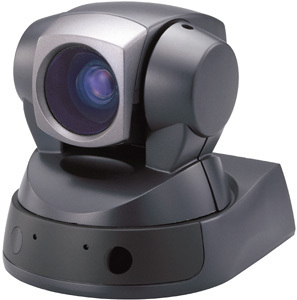
\includegraphics[width=1.6in]{images/ptz_front}
				\caption{Front side.}
			\end{subfigure}
			\qquad
			\begin{subfigure}[h]{0.4\linewidth}
				\centering
				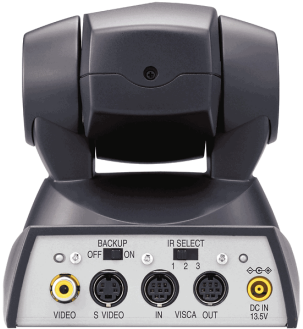
\includegraphics[width=1.6in]{images/ptz_back}
				\caption{Back side.}
			\end{subfigure}
			\caption{Sony EVI D100P.}
			\label{fig:3_evi}
		\end{figure} 
		
		The first hardware element that we used is the Sony EVI D100P\footnote{\url{https://pro.sony/en_IN/products/ptz-network-cameras/evi-d100-d100p-pal-}}. It is a \emph{PTZ} cam (which stands for \emph{Pan Tilt Zoom}). It is a camera which, originally thought and designed for videoconferences, is equipped with a bunch of precision motors. This allows it to be teleoperated, performing a soft and steady two-dimensional movement on demand:
		\begin{itemize}
			\item \emph{Pan:} horizontal movement. It can take values from $-164º$ to $164º$ from the centered position. This movement can be performed at a certain speed, which can be setted between $1$ and $24$.

			\item \emph{Tilt:} vertical movement. Its range goes from $-30º$ to $30º$, and the movement speed can be also varied between $1$ and $20$.
		\end{itemize}

		The low-level implementation of the movement commands is the \emph{VISCA} protocol, a propietary solution from the manufacturer (Sony). It is received by the cam through a RS-232C (the traditional low-rate serial interface before USB extended), so we can connect it to a modern computer with a RS232-USB interface.

		However, the driver that controls this camera (\ref{sec:3_evicam_driver}) does not offer support for a \emph{zoom} movement, but it is not very relevant for this application.\\

		As the video sensor is an analogue device, we need to convert it to a digital format. We achieve this with a video capture device, which outputs video in a digital format. This image flow will be processed by a ROS driver (\autoref{sec:3_usb_cam}), that will be later explained.\\

		Something remarkable about this device is that it is a bidirectional device: we \textit{receive} images from its camera, and, at the same time, we \textit{send} it commands to move the motors.\\
		
		As we can infer from the described technical specifications, this is a relatively old device, so we have to be careful on the movement commands. This is due to the short period of position update: even if we command the motion action at the maximum available speed, the movement won't complete before the next update is commanded. In addition, the camera mantains a buffer of the pending commands to be updated. Hence, sending absolute movement commands (\autoref{fig:3_ptz_wrong}) will result in a chaotic behavior of the camera.\\
		
		So, we have needed an alternative approach, consisting of \emph{differential} movements (\autoref{fig:3_ptz_right}). This has the objective of ensuring its completion before the next iteration comes in, so we will perform it at the maximum available speed.

		\begin{figure}[h]
			\centering
			\begin{subfigure}[h]{0.4\linewidth}
				\centering
				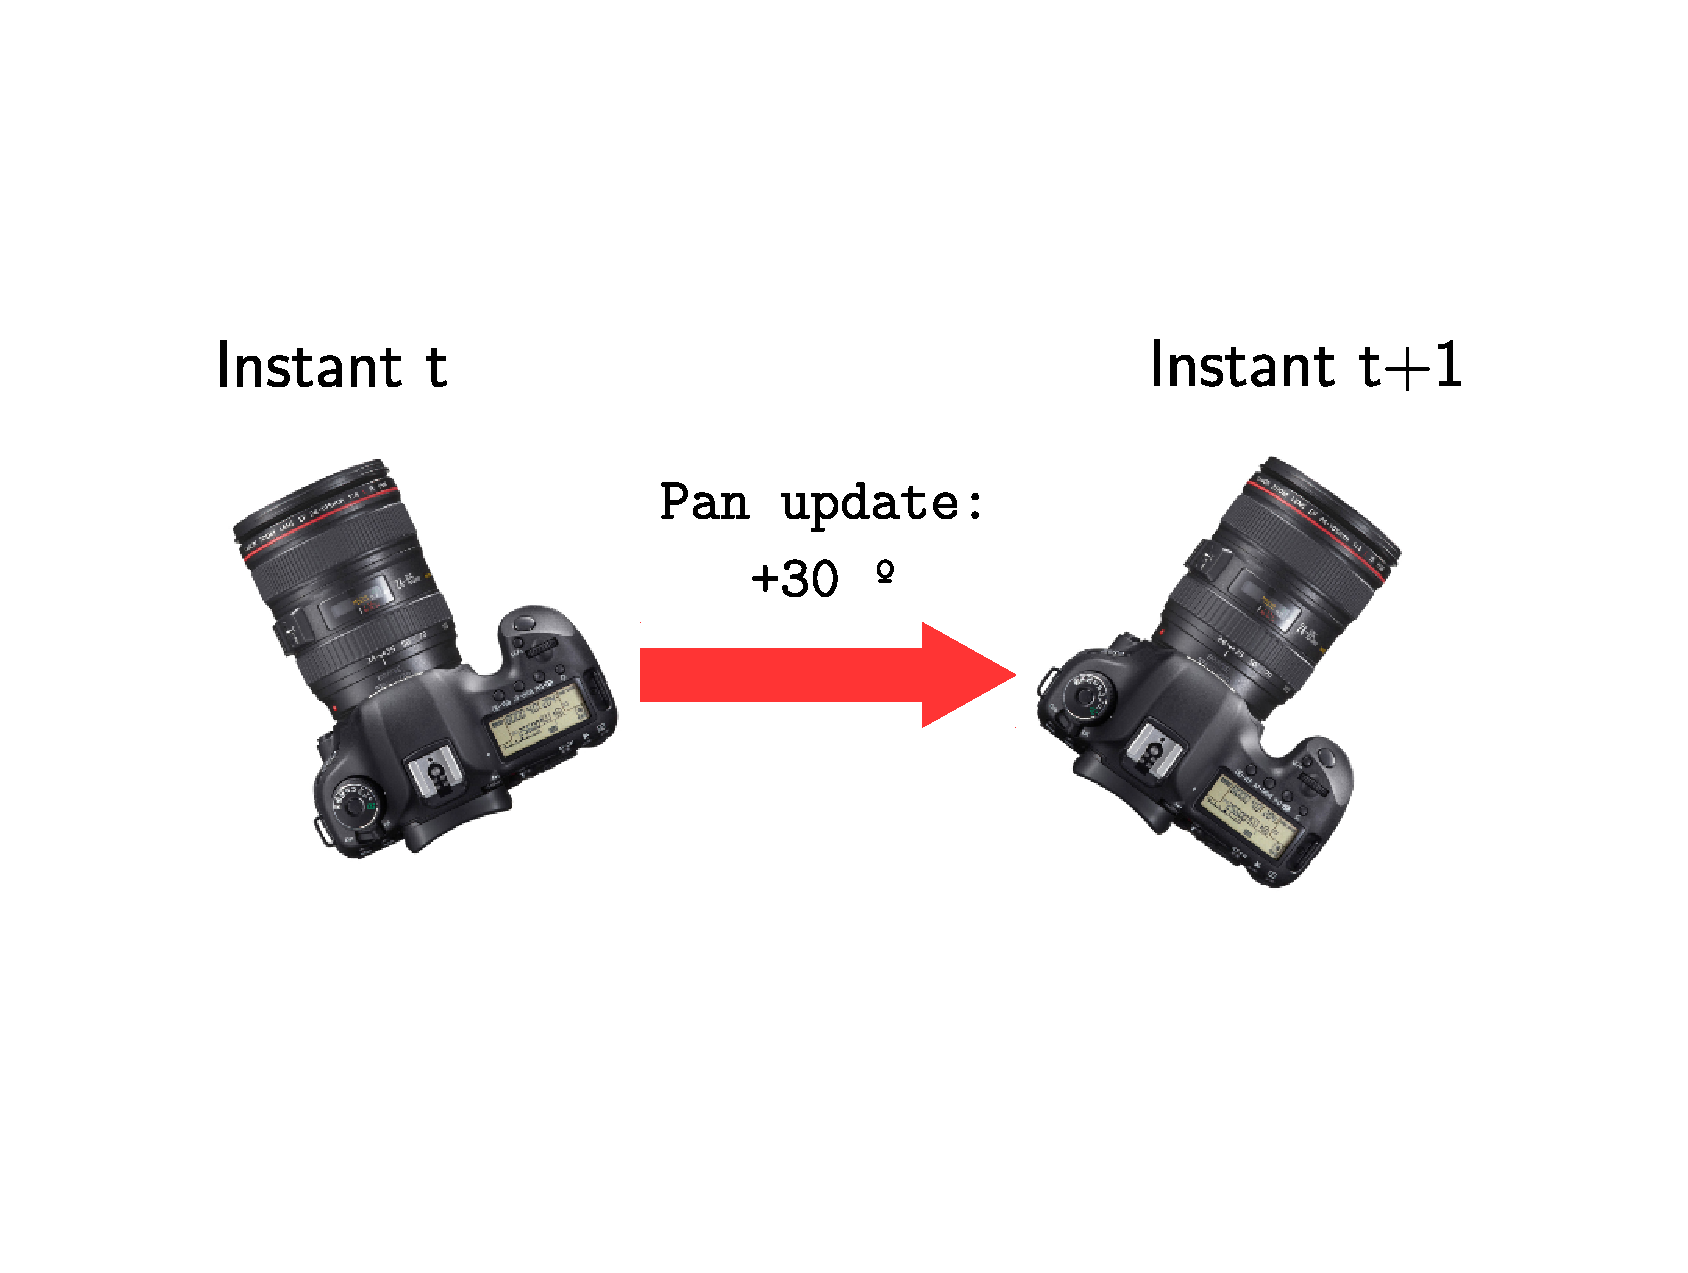
\includegraphics[width=2.7in]{images/ptz_wrong_movement}
				\caption{Wrong motion update (too long movements).}
				\label{fig:3_ptz_wrong}
			\end{subfigure}
			\qquad
			\begin{subfigure}[h]{0.4\linewidth}
				\centering
				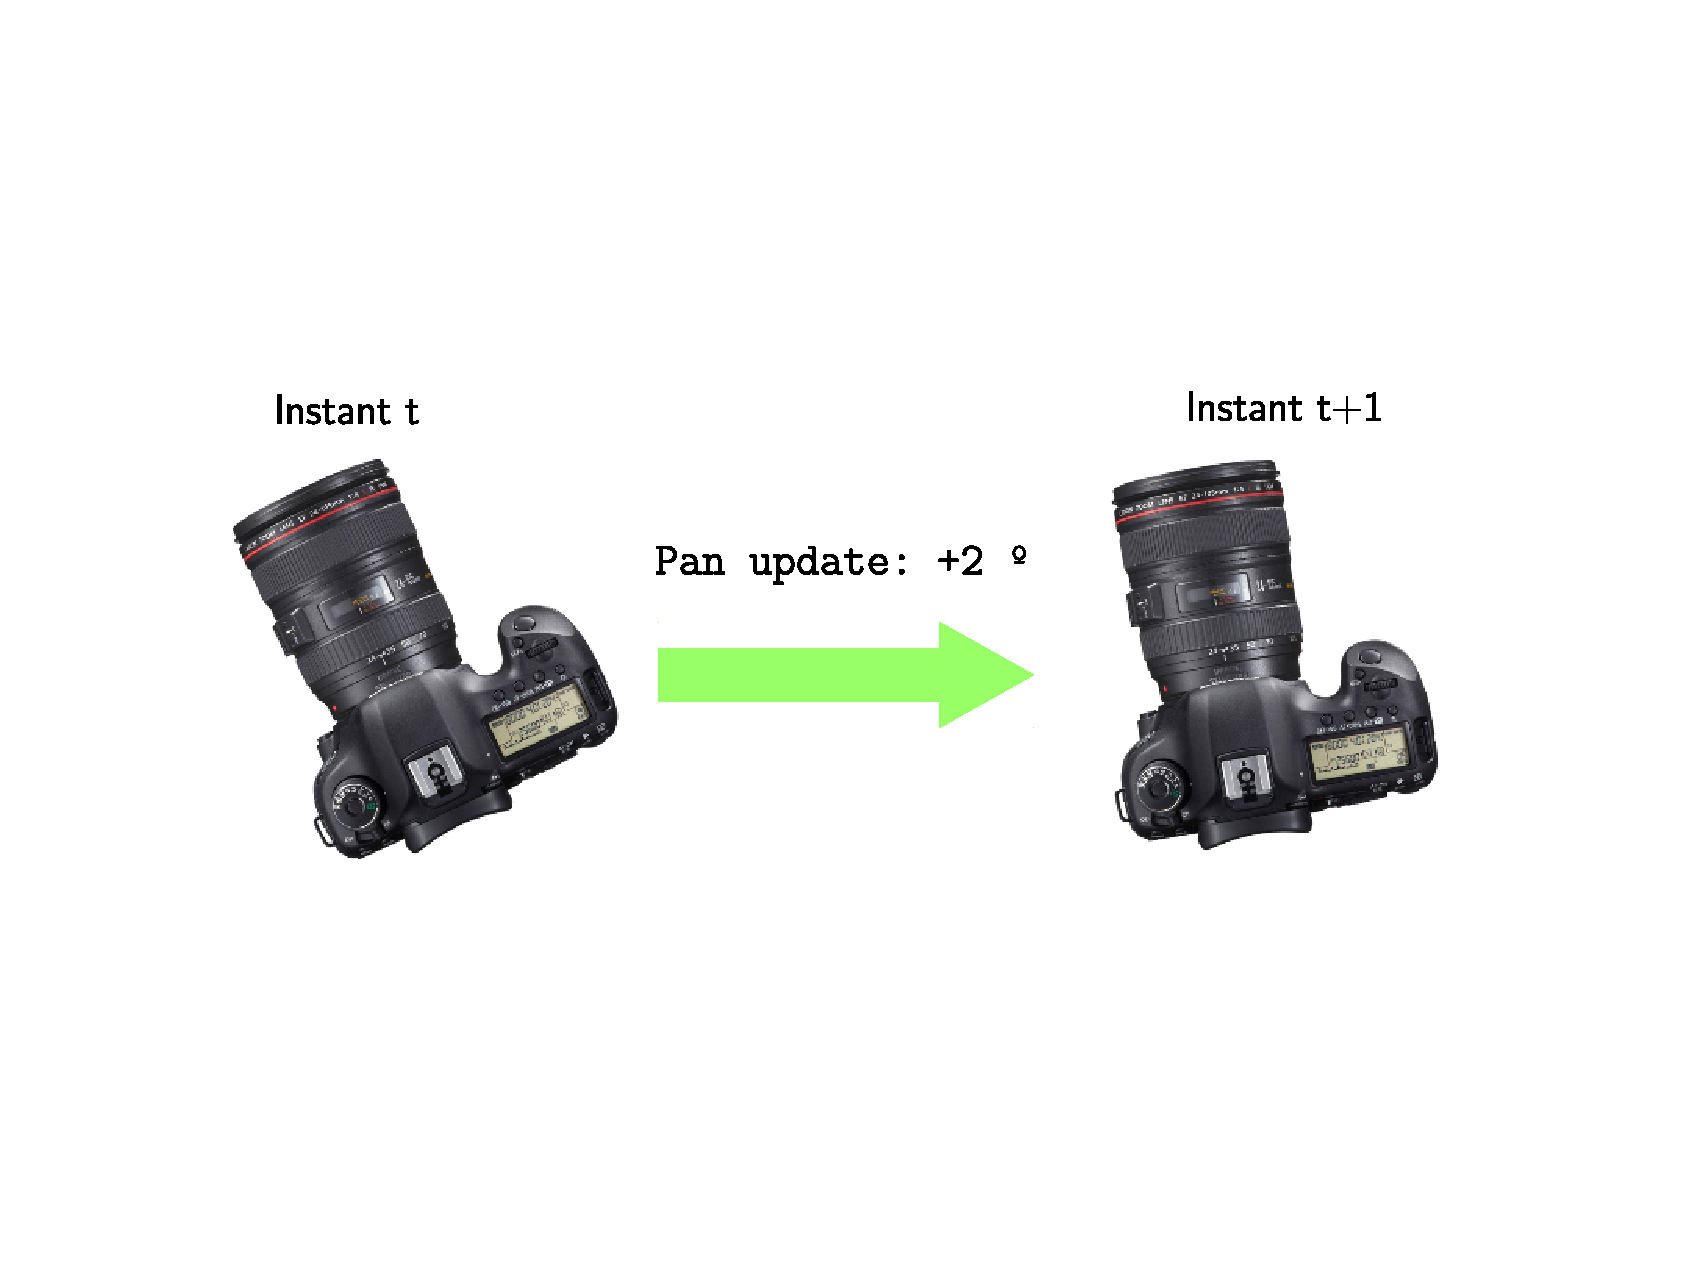
\includegraphics[width=2.7in]{images/ptz_correct_movement}
				\caption{Correct motion update (short differential movements).}
				\label{fig:3_ptz_right}
			\end{subfigure}
			\caption{Comparison between possible approaches for Pan/Tilt angle updates.}
			\label{fig:3_ptz_movements}
		\end{figure}
		

		This was the device we used for our first approximation to the sensing+actuating node (\autoref{sec:follow_ptz}), where the only response was moving the camera.\\

	\subsection{Asus Xtion Pro Live}
		It is a RGBD (RGB + Depth) sensor, designed by Asus for interactive PC applications development purposes. \\

		It has been our image source in the sensing+actuating node (\autoref{sec:follow_turtlebot}) we have developed. We used it in the second approximation (the response was the movement of the entire robot).

		\begin{figure}[h]
			\centering
			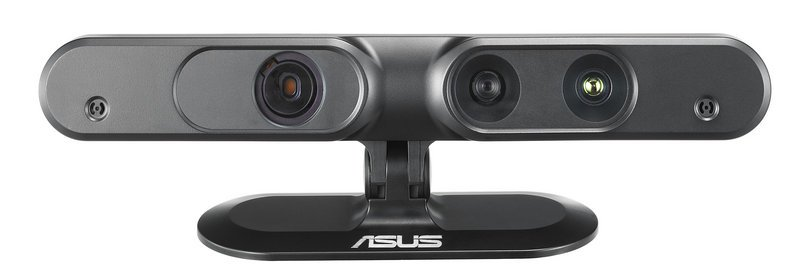
\includegraphics[width=0.4\linewidth]{images/xtion}
			\caption{Asus Xtion Pro Live. IR emitter (left), and RGB and IR lenses (right).}
			\label{fig:3_xtion}
		\end{figure}

		It counts on the left side with an IR (\emph{infrared}) light emitter, which radiates beams like a conventional light bulb (that's its function).\\

		On the right side, we can find two sensors:
		\begin{itemize}
			\item \emph{RGB sensor:} a conventional digital camera, with a resolution up to 1280x1024 px.
			
			\item \emph{Depth sensor:} it is capable of measure distance to objects, by receiving the reflections of the IR beams that we have mentioned above. It maps, for each pixel, the distance to that reflection (in mm), stored as a 16-bit long value.\\
			
			Thus, we can obtain a depth image, with a resolution of 640x480 px (@ 30 fps).
		\end{itemize}
		
		As it can be seen on \autoref{fig:3_xtion}, both sensor can't physically be in the same place, so there is a little discrepancy between both computed images:

		\begin{figure}[h]
			\centering
			\begin{subfigure}[h]{0.4\linewidth}
				\centering
				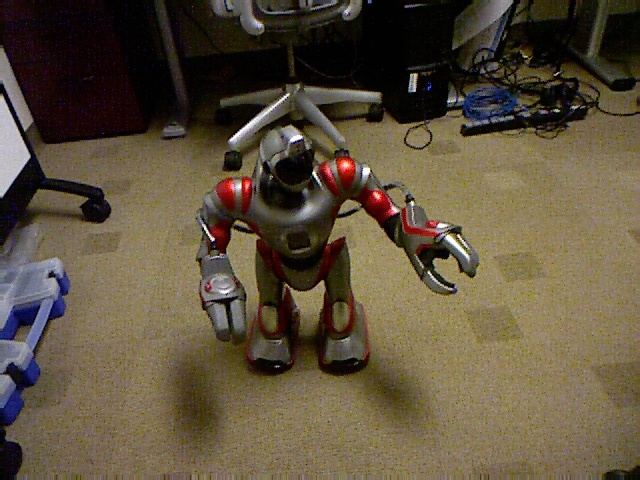
\includegraphics[width=3in]{images/rgb_before}
				\caption{RGB image.}
				\label{fig:3_rgb_bef_reg}
			\end{subfigure}
			\hfill
			\begin{subfigure}[h]{0.4\linewidth}
				\centering
				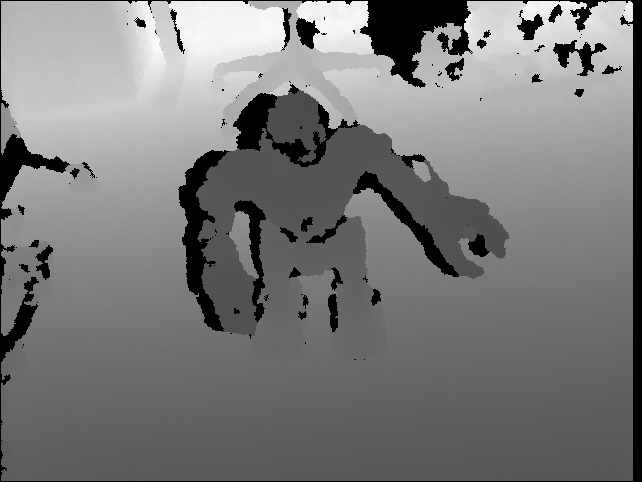
\includegraphics[width=3in]{images/depth_before}
				\caption{Depth image.}
				\label{fig:3_depth_bef_reg}
			\end{subfigure}
			
			\begin{subfigure}[h]{0.9\linewidth}
				\centering
				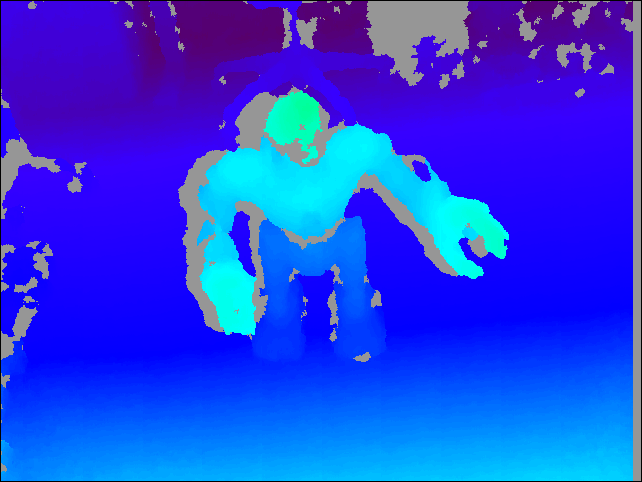
\includegraphics[width=3in]{images/disparity_before}
				\caption{Disparity (difference) between \ref{fig:3_rgb_bef_reg} and \ref{fig:3_depth_bef_reg}.}
				\label{fig:3_disparity_bef_reg}
			\end{subfigure}
			
			\caption{Both images sensed by the Xtion cameras, and the disparity between them \emph{before} the registration process.}
			\label{fig:3_bef_reg}
		\end{figure}
		
		With the goal of paliating this disparity, a process called \emph{registration} is executed for every new incoming depth image. It consists of a projection of the depth pixels into the RGB image, trying to align on an optimum way each pixel with its counterpart on the RGB image. We can observe that this can cancel to some degree the difference between both images (\autoref{fig:3_aft_reg}).
		
		
		\begin{figure}[h!]
			\centering
			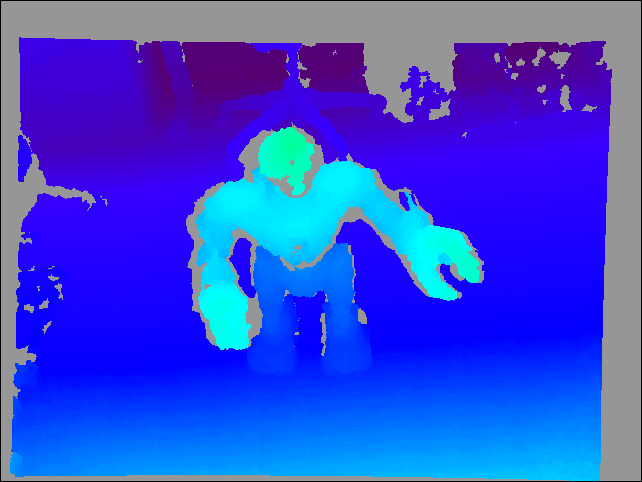
\includegraphics[width=3in]{images/disparity_after}
			\caption{Disparity between the images \emph{after} the registration process.}
			\label{fig:3_aft_reg}
		\end{figure}
		
		If we compare the new disparity (\autoref{fig:3_aft_reg}) with the previous disparity (\autoref{fig:3_disparity_bef_reg}), we can appreciate that now, the RGB and Depth images are aligned on an improved way, as if both sensors were on the same place, or much closer at least.\\
		
		So, from now on, we will call \emph{depth image} to the registered version of the depth map, as the unregistered image is not useful anymore.\\
		
		At last, we will make a mention to the open source drivers\footnote{\url{https://structure.io/openni}}, OpenNI (\emph{Open Natural Interaction}). They were originally developed by the Kinect developer company PrimeSense (which designed the Xtion device beside Asus).\\
		
		This interface allows to perform all the processes involved into handling this device (image grabbing, depth registration, etc.).
		
	\subsection{Turtlebot 2}
		The Turtlebot platform has been our main actuation platform on the developed actuation+response node (\autoref{chap:followperson}).\\
		
		\begin{figure}[h]
			\centering
			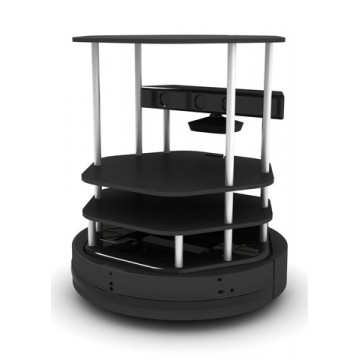
\includegraphics[width=3in]{images/turtlebot}
			\caption{Turtlebot development kit.}
			\label{fig:3_turtlebot}
		\end{figure}
		
		It is a research platform, composed by a structure jointed to a Kobuki robot (mobile base)\footnote{\url{http://kobuki.yujinrobot.com/about2/}}. Into this structure, there are also attached an Asus Xtion sensor (recently described), and a laser sensor, which has not been used on this project (nevertheless, it could be a continuation, as a navigation algorithm could be added to this project, on a similar way than in \cite{rocapal}).\\
	
		The user has the capability of connecting each of these devices via USB to the laptop, and place it at the top platform of the robot. From there, the computer can run the algorithm and command the movements. Every component can be handled with the respective ROS driver (which will be described later).
	

\section{Python}
	According to the official definition from \cite{python}, Python is \textit{an interpreted, object-oriented, high-level programming language with dynamic semantics}. It was created in 1991 by Guido van Rossum (who consecrated its name to the TV series \textit{Monty Python}). However, due to the increasing growth of \emph{Machine Learning} that happened the last two decades, it has become the most popular language for this purpose, due to its focus on \emph{easiness}, its duck typing\footnote{This refers to Python guessing about your variables, coming from the phrase \textit{''if it looks like a duck and sounds like a duck, chances are it's a duck."}} and its strong Object Orientation: everything can be treated as an object on this language. This is a very interesting feature, as it facilitates features as sharing memory, abstract processes, and much more.
	
	And, of course, it is \textit{Open Source}, so it is always under community improvements, and there are a vast number of incredibly useful third party libraries, which are impossibly easier to deploy onto your code.\\
	
	This makes this language a really potential candidate for the applications to develop (and that's precisely the reason that explains its huge growth on the software market).\\
	
	For our target, we will use Python on its version $2.7$. Although it is a relatively old version of the language, it is necessary to mantain the compatibility with ROS (\autoref{sec:3_ros}) bindings, which have not still taken the leap to the newest major version ($3.x$) on Python.\\
	
	Nevertheless, we want to mention the fact that Python is an \emph{interpreted} language, which means that its sentences are projected on another program (the Python interpreter, which executes them), and not directly by the processing hardware (CPU/GPU). This can be a con, as it makes the code execution much slower, in comparison with standard \emph{compiled} languages, which are run directly as processes, and taken by the computer hardware for its execution (as C, C++, Picky, etc.).

\section{ROS}
	\label{sec:3_ros}
	As it is said on \cite{ros-intro}, \emph{ROS} (Robot Operating System) is \textit{an open-source, meta-operating system for your robot}, maintained by the \emph{OSRF} (Open Source Robotics Foundation). It is a framework that provides a distributed, easily-scalable environment of \emph{nodes}. These nodes are programs which are independently running on the computer (or distributed over a P2P network), so they can perform individual tasks. However, they can communicate between themselves on a synchronous way (over \emph{services}, implementing a client-server role system between nodes), or on an asynchronous way, via \textbf{topics}, which will be the main benefit we will take advantage of. These topics, which rely on a standard TCP/UDP communication between sockets via the \texttt{loopback} interface, are intended for an unidirectional, streaming communication, where a node can take a role: \emph{publisher} (if it is writing data inside the topic), or \emph{subscriber} (if it is reading the data that publishers are broadcasting into the topic). The data flow through the topic, however, is not unrestricted. It must follow a ROS specific syntax, the \emph{Message} type, which is strictly defined for the communication purpose (geometry, sensoring, etc.).\\
	
	For our project we will be using the 2016 \textit{LTS} (Long Term Support) version, called \textit{Kinetic Kame}\footnote{\url{http://wiki.ros.org/kinetic}}. This is the version bundled on the installation of JdeRobot\footnote{\url{https://jderobot.org/Installation}}.\\
	
	ROS provides libraries and bindings for C++, Lisp, and \textit{Python} (\texttt{rospy}). They allow, among plenty of other stuff, to really easily set up a topic between two or more programs, which will be seen as ROS nodes.\\
	\begin{figure}[h]
		\begin{lstlisting}
...
import rospy
from std_msgs.msg import String
...
rospy.init_node('listener')              # Starting the node entity.
rospy.Subscriber('chatter', String)      # Instantiation of the topic subscriber.
rospy.spin()                             # 'Infinite loop' listening to the topic.
...
		\end{lstlisting}
		\caption{Simple stablishment of a listener node through \texttt{rospy} (code from \cite{listener-rospy}).}
		\label{fig:3_rospy_listener}
	\end{figure}
	
	However, this topic communication will be abstracted on our project by the \texttt{comm} library, as it will be seen on \autoref{sec:3_comm}.\\
	
	ROS also provides a Debian package, called \texttt{rosbash}, which allows to, in a very handy way, manage nodes and packages from a standard \texttt{bash} shell. The most remarkable feature for us is the command \texttt{roslaunch}, that launches a ROS node with a certain specific settings, configurable via a \texttt{.launch} file (which follows a XML formatting). An example for the file structure can be found on \autoref{fig:3_launch_file}.\\
	
	\subsection{\texttt{usb\_cam}}
	\label{sec:3_usb_cam}
		ROS node that creates a topic and publishes into it the digital video data incoming from a USB camera, into the topic \texttt{/usb\_cam/image\_raw}.\\
		
		This node will be used on the first approach to the sensing+actuating node (\autoref{sec:follow_ptz}), with the purpose of retrieving images from the Sony EVI D100P camera (\autoref{fig:3_evi}). In consequence, a custom configuration file\footnote{\url{https://github.com/RoboticsURJC-students/2017-tfg-nacho\_condes/blob/master/resources/usb\_cam-test.launch}} is required. We can have a glance on that configuration file (\autoref{fig:3_launch_file}).\\
		
		\begin{figure}[h]
			\centering
			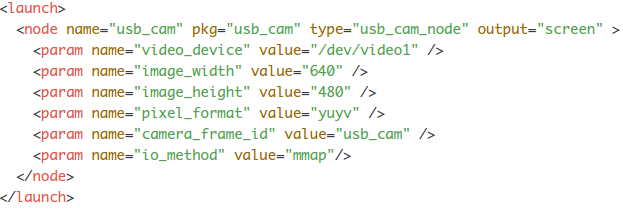
\includegraphics[width=5in]{images/usb_cam_test}
			\caption{Example of \texttt{usb\_cam-test.launch} configuration file for a ROS node.}
			\label{fig:3_launch_file}
		\end{figure}
		\begin{center}
			Usage: \texttt{roslaunch usb\_cam-test.launch}
		\end{center}

	\subsection{\texttt{openni2\_launch}}
		This ROS binding \cite{openni2-doc} provides the launch files for the \texttt{rgbd\_launch} node. This node publishes on several topics the RGB+D images provided by the Asus Xtion (\autoref{fig:3_xtion}), performing at the same time the registration process.\\
		
		This node will be used on the second iteration of the sensing+actuating node (\autoref{sec:follow_turtlebot}). It will connect the Xtion sensor to the component, providing the real-time imaging through the topic.\\

		\begin{center}
			Usage: \texttt{roslaunch openni2\_launch openni2.launch}
		\end{center}
		

	\subsection{\texttt{kobuki\_node}}
		This ROS package contains a bunch of launch files. Among them there is the one we will use: \texttt{minimal.launch}, which starts the \emph{nodelet}\footnote{A ROS nodelet performs multiple simultaneous processes, and consequently opens several topics.} that gives us the total control of the Kobuki robot connected to the computer\footnote{We refer to the robot as \emph{Kobuki} now because the mobile base of the Turtlebot (\autoref{fig:3_turtlebot}) is the only ROS device which we will control in our application.}.\\
		
		This node will be used on the second iteration of the sensing+actuating node (\autoref{sec:follow_turtlebot}). It will connect the Turtlebot motors to the component, providing the topic to command movements to them.
		
		\begin{center}
			Usage: \texttt{roslaunch kobuki\_node minimal.launch}
		\end{center}

	
\section{JdeRobot}
	As described in \autoref{sec:dl_jderobot}, JdeRobot\footnote{\url{https://jderobot.org}} is a distributed development platform/middleware, born in \cite{jmplaza-phd}. It stands out mainly for two key aspects:
	\begin{itemize}
		\item \textit{Hardware abstraction:} it behaves as an intermediate layer between control software (written by the programmer) and hardware, which can be a real device (a robot, drone, camera, laser scanner, etc.), or a simulation (on the open source world simulator Gazebo\footnote{\url{http://gazebosim.org/}}). This way, the bidirectional flow (information from sensors, and commands from the computer) is sent the same way, \textit{no matter the kind of the robotic device}.
		
		As well, this abstraction layer allows various computers to interact simultaneously with the hardware, as the communications are also abstracted to ROS topics or ICE endpoints (it will be properly explained at \autoref{sec:3_comm}), where a program has to just listen/talk to be in on. This provides a very valuable \textit{software and hardware scalability to the platform, and to the developed programs}.\\
		
		Let's have a look on a possible example on the \autoref{fig:3_jderobot_hal}. This could represent an scenario where somebody wants to virtually test a navigation algorithm. Thus, in the \emph{Computer 1}, a reactive controller is running, sensing the environment through a real laser scanner and a RGB camera (as in the work developed at \cite{rocapal}). This controller receives data from the sensors, computes a proper navigation response, and sends it to a virtual robot, simulated on Gazebo.
		
		Additionally, another machine (\emph{Computer 2}) is running a viewer, which allows it to draw the images seen by the camera, and the laser readings from the scanner. So, this component only receives the data from the sensors, and does not send any kind of data to the devices.
		
		We can see that both components can perfectly run together and on different machines, even when they are written over completely different languages (Python and C++, respectively). In addition, we can perfectly handle virtual and real devices simultaneously, even if they talk through different interfaces (ROS or ICE), due to the perfect support of this division by the \texttt{comm} (\autoref{sec:3_comm}) library.\\
		
		
		\begin{figure}[h!]
			\centering
			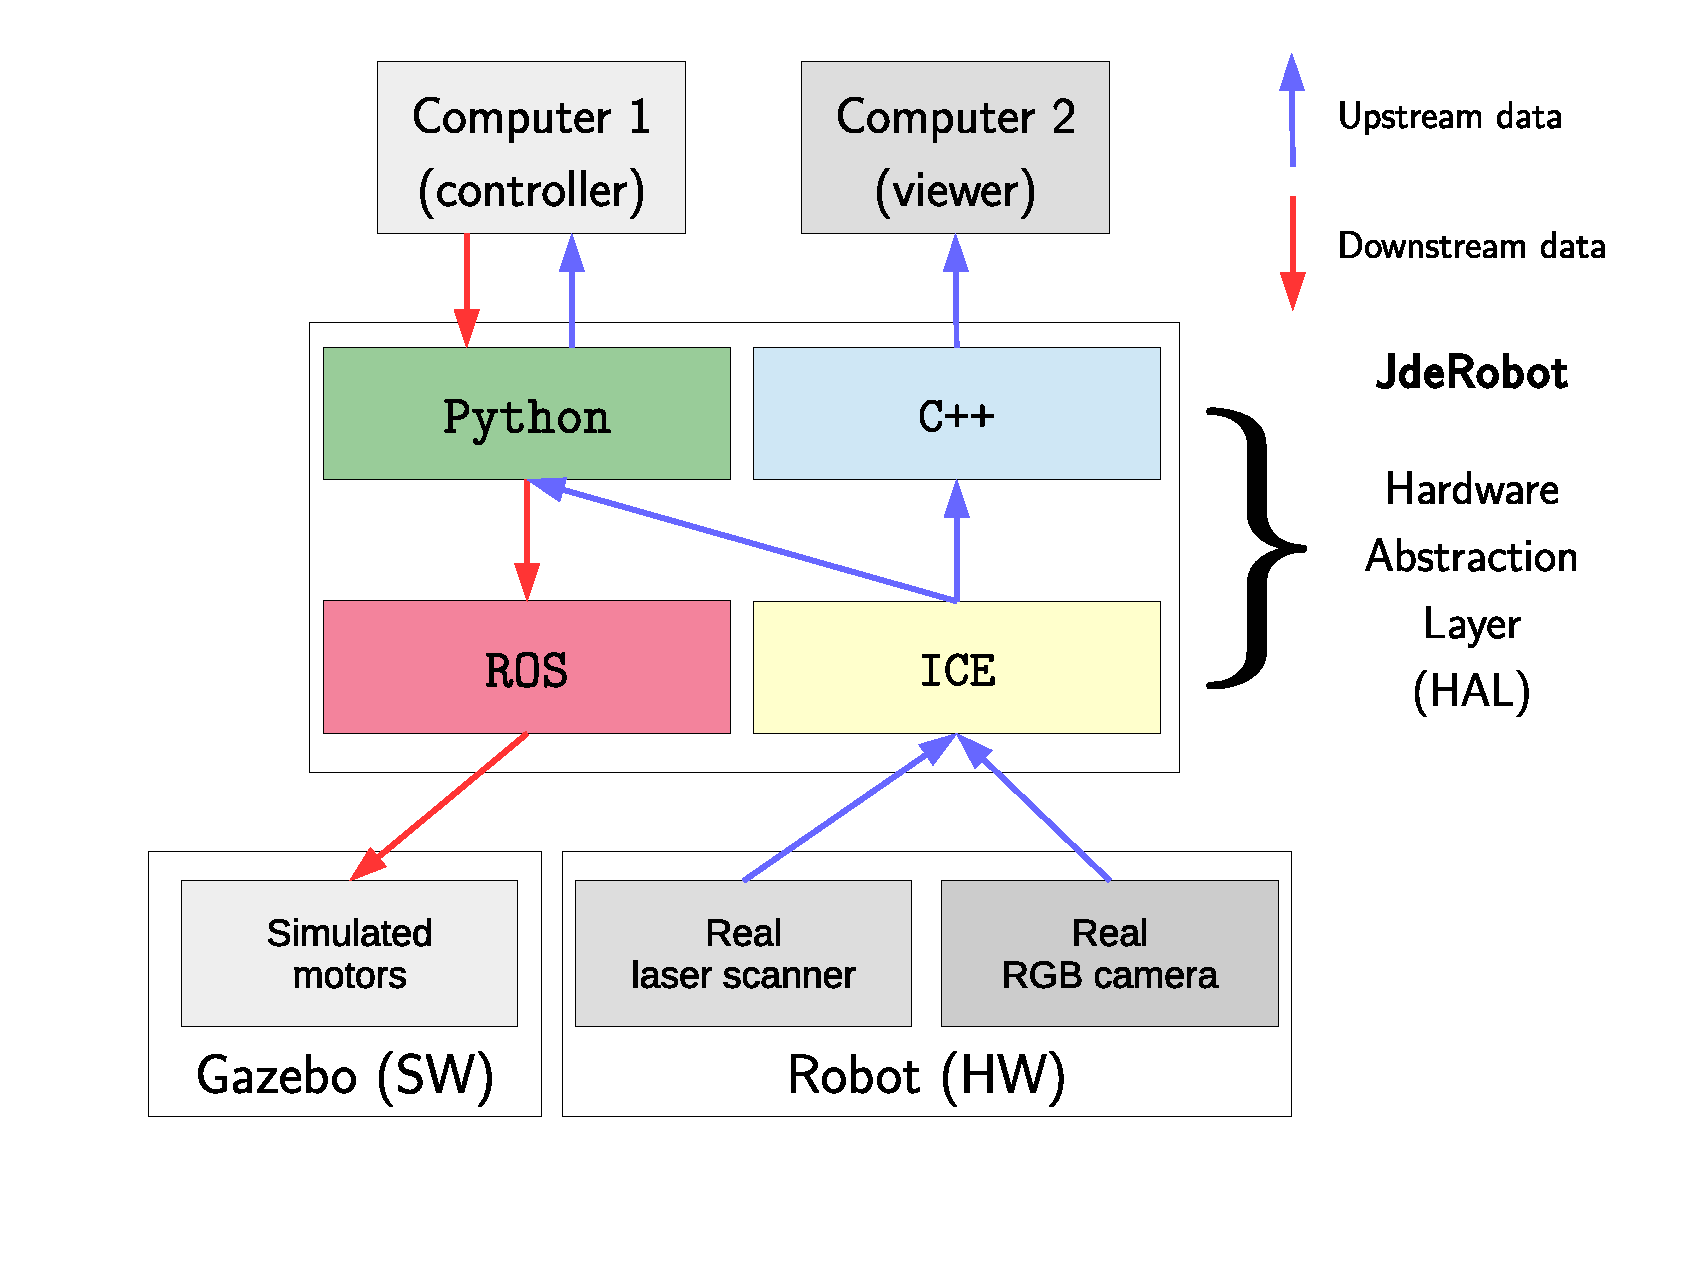
\includegraphics[width=4in]{images/jderobot_hal}
			\caption{JdeRobot abstraction layer, and a possible use distributed, multi-middleware scenario.}
			\label{fig:3_jderobot_hal}
		\end{figure}
		
		 \textit{So, in this easiness and flexibility resides the main advantage of using JdeRobot}.
		
		\item \textit{Wide device support:} JdeRobot provides full compatibility with ROS Kinetic Kame, so it can perfectly integrate with ROS Nodes (in our concern, we can communicate with the Turtlebot and the Xtion devices via several topics that the ROS intermediate nodes open).
		
		\item \textit{Behavioral based on threaded parallel schemes:} as it is introduced at  \cite{jmplaza-phd}, inside a component, we will find one or more \emph{schemes}, objectified on threads. These threads run concurrently with an specific timing (so it does not overload the CPU in vain if a few iterations per second are enough for a vivacious and correct response).\\
		
		These schemes perform different tasks each, as seen on \autoref{fig:2_tasks} on a non-blocking way, and share memory. This has been followed on a comfortable way on our implementation: the threads are independent, but the tasks they control are performed by Python objects, which are interconnected between them:
		
		As an example, we can see how this has been performed inside our Python code:
		
		\begin{figure}[h]
			\centering
			\begin{lstlisting}
...
cam = Camera(ros_topic)           # Creation of the camera.
net = Network(graph_model)        # Creation of the CNN.

net.setCamera(cam)                # Connection of the camera and the CNN,
                                  # which now can share memory.

t_cam = ThreadCamera(cam)         # Instantiation and start of the thread which
t_cam.start()                     # implements the Camera schema.

t_net = ThreadNetwork(net)        # Instantiation and start of the thread which
t_net.start()                     # implements the Network schema.
...
			\end{lstlisting}
			\caption{Handling schemes on Python with objects and threads.}
			\label{fig:3_schemes_python}
		\end{figure}
	\end{itemize}
	
	\vspace{0.4in}
	
	To sum up, we have described the goodness of the JdeRobot framework for our purposes, and seen how we can implement the \textit{useful schemes paradigm} on an easy way into Python, our development language.\\
	
	Now, in the next subsections, we will examine which of the JdeRobot components, apart of the structure, have been of greatest interest for us.
	
	\subsection{Digit Classifier}
	\label{sec:3_digitclassifier_jderobot}
		This JdeRobot component\footnote{\url{https://github.com/JdeRobot/dl-digitclassifier}} was originally designed by David Pascual \cite{dpascualhe} and Nuria Oyaga \cite{noyaga}, and it was used on this project to land on the concept of neural networks.\\
		
		Its design aims to \textit{classify handwritten numbers} with the use of a Convolutional Neural Network (\autoref{sec:1_cnn}), that classifies the incoming images from a video source.\\
		
		\begin{figure}[h]
			\centering
			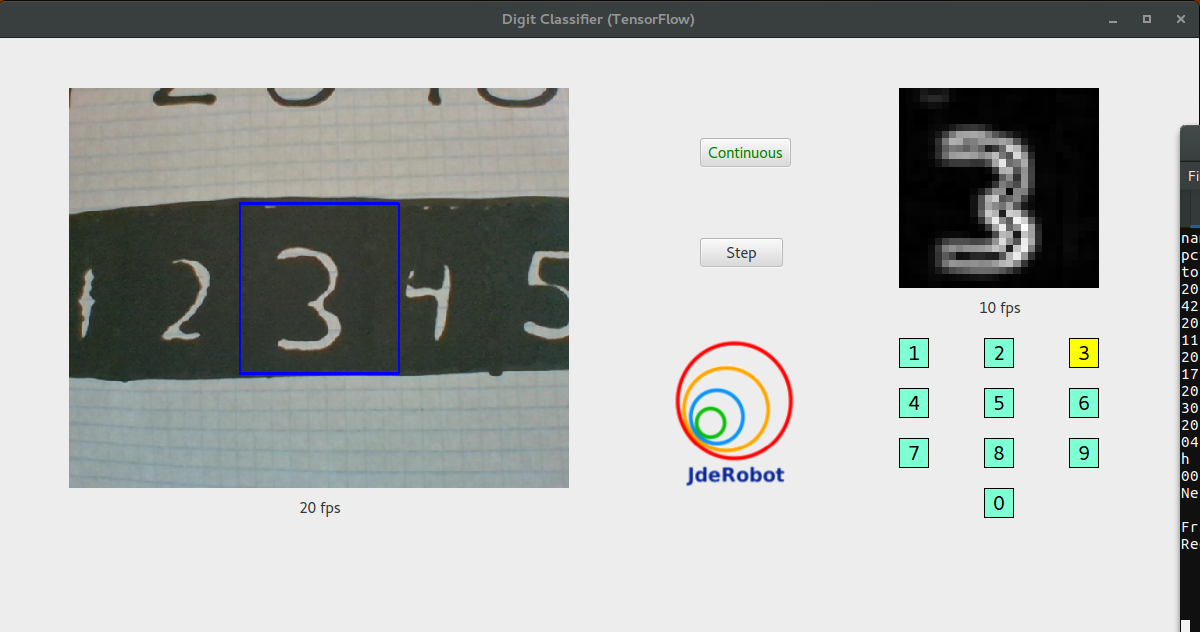
\includegraphics[width=4in]{images/digitclassifier}
			\caption{\texttt{DigitClassifier} on action.}
			\label{fig:3_digitclassifier}
		\end{figure}
		
		The previous implementations were written in Keras and Caffe (Python libraries to implement Neural Networks), so we made the same on TensorFlow (\autoref{sec:3_tensorflow}), to accomplish an initial domain of this Machine Learning framework.\\
		
		The implementation of this convolutional neural network consists on a concatenation of layers, following the scheme shown on \autoref{fig:3_digitclassifier_neural_structure}, which perform specific operations.
		
		\begin{figure}[h]
			\centering
			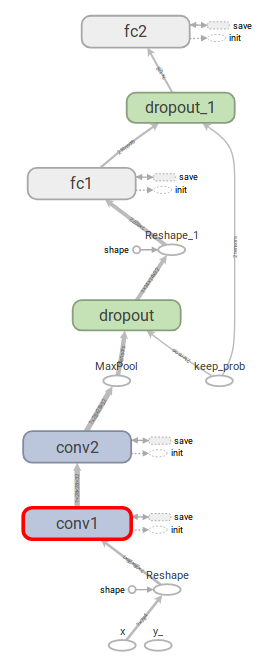
\includegraphics[width=2in]{images/digitclassifier_network_graph}
			\caption{Digit classifying neural structure.}
			\label{fig:3_digitclassifier_neural_structure}
		\end{figure}



		\begin{enumerate}
			\item \texttt{conv1}: first convolutional layer. As described in \autoref{sec:1_cnn}, it performs a 2D convolution between a $5px \times 5px$ square mask\/kernel (\texttt{W\_conv1}), and then adds a bias/intercept term (\texttt{b\_conv1}).\\
			\item \texttt{conv2}: second convolutional layer. It performs the same operation taking the output from the previous layer as an input, using a different weights mask and bias terms.\\
			
			Until now, what we have done is extracting patterns on each digit type (e.g. discovering typical circles on $0$ and $8$, which are always present on the same zone of the image).\\
			\item \texttt{pooling}: as the activation maps can be growing in size as we perform feed forward propagation, a \emph{pooling} operation is performed. It consists on sampling the input. Concretely, we retain the \textit{maximum} value for each 2 pixels, which is known as \textit{$2x2$ \texttt{max pooling}}
			
			\item \texttt{dropout}: this layer does not strictly perform any mathematical operations. It lets pass the TENSORS through it, but randomly switching off some neurons. This is parameterized by a user input, using a variable called \texttt{keep\_prob}. In our case, we set it to $0.5 (50\%)$ during the training process, to avoid overfitting by forcing the network to modify the neural paths randomly, as not every neuron is available on every moment. This is kind of similar to augmenting the dataset during the training process. The rest of the time (when the network is used to make inferences), this parameter is set to $1.0$, which means that no neurons are switched off at all.\\
			\item \texttt{fc1}: first fully connected layer. These layers, also known as \emph{dense} layers, are distinguised because every neuron is connected to every activation from the previous layer. So, this kind of layers are used for \text{pattern association with labels}, due to the relationship they can infer between every input.\\
			\item \texttt{fc2}: the output layer. It connects all the outputs of the previous dense layer and groups the output in a 10-dimensional vector, which contains the probability of the digit to belong to each one of the possible classes.
		\end{enumerate}


		
		Once all this was achieved, we upgraded the code (from single ICE support to ROS+ICE via the \texttt{comm} library), and unified it (Keras + TensorFlow frameworks in a single component, under choice using the YML configuration file) on the official JdeRobot repository. From there it can be used right out of the box with the included model for both frameworks. In addition, you can train your own models using the provided datasets, or yours if you build another.
	
	
	\subsection{\texttt{evicam\_driver}}
	\label{sec:3_evicam_driver}
	This driver, bundled into JdeRobot\footnote{\url{https://github.com/JdeRobot/JdeRobot/tree/master/src/drivers/evicam\_driver}}, allows the user to send movements commands to a Sony EVI D100P camera \autoref{fig:3_evi}) and retrieve information from it, creating an ICE endpoint that is ready to interact with the camera \emph{PT} (Pan, Tilt) motors.\\
	
	As this is a low-level driver, written in C++, it requires to be used on a specific way, which has been documented\footnote{\url{https://jderobot.org/Handbook\#PanTilt_Teleop}} to be easily applied in the future.\\
	
	This driver defines an interaction API with the camera, which allows us to get the values from the motors encoders:
	\begin{lstlisting}
import config
import comm
...

cfg = config.load('yml_configuration_file')
jdrc = comm.init(cfg, 'NodeName')


# Instantiation for the motors:
PTMotors = jdrc.getPTMotorsClient('NodeName.PTMotorsEndpoint')

print(PTMotors.getLimits()) # Shows the max/min values for pan, tilt 
                            # and each speed.

print(PTMotors.motors.data) # Shows the current values for pan, tilt
                            # and each speed.

# Let's move the camera! As easy as:
PTMotors.setPTMotorsData(new_pan, new_tilt, max_pan_speed, max_tilt_speed)
	\end{lstlisting}
	
	\subsection{\texttt{comm}}
		\label{sec:3_comm}
		\texttt{comm} is the basic library to perform communications between different components. It is what supports all the data flows in a typical scenario (\autoref{fig:3_jderobot_hal}).\\
		
		\texttt{comm} consists on a collection of bindings to easily create a link between two components, or between a device and a component. On the lowest level, we can use it relying on ROS (through topics as it was explained before on \autoref{sec:3_ros}), or through an ICE proxy. ICE\footnote{\url{https://zeroc.com/products/ice}} is an object-oriented middleware that, in our purpose, allows to abstract a data flow to a TCP/IP endpoint (an address/hostname, and a port), which can even support a communication between two or more programs inside the same machine.\\
		
		To create a communicator with \texttt{comm}, it needs the specification for that link (underlying middleware, topic/endpoint, etc.), so it uses the JdeRobot standard: YML\footnote{Legible data serialization format.} configuration files, which can be like in \autoref{fig:3_yml_format}.
		\begin{figure}[h]
			\centering
			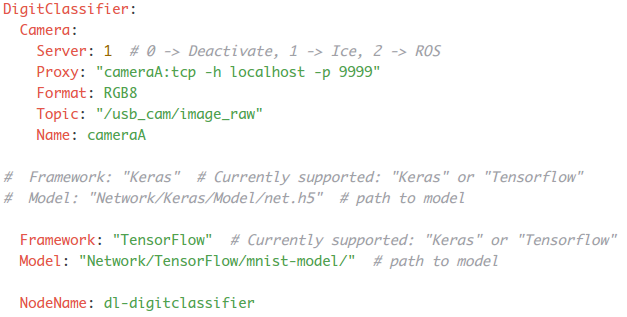
\includegraphics[width=4in]{images/yml_format}
			\caption{YML format on the \texttt{digitclassifier.yml} file.}
			\label{fig:3_yml_format}
		\end{figure}
		
\section{OpenCV}
\section{TensorFlow}
\label{sec:3_tensorflow}
\section{Keras}
\section{PyQt (v.5)}
\section{Threading}


% ---- Perception module ----
\section{Perception Module}

This module is responsible for apprehending the incoming images (RGB and depth) from the sensor, and generates a significant output to be interpreted by the actuation module. Its structure follows a certain pipeline with five steps (Figure \ref{fig:infra_scheme}): image acquisition, person detection, face detection, person and face trackers, and face reidentification. This pipeline allows the system to discern if the target person is being seen right now. 

\subsection{Person Detection}

First, the incoming RGB images are passed through an \emph{object detection} module. It is powered by a pretrained CNN, which has a special architecture designed in \cite{ssd} for this purpose: SSD (\emph{Single-Shot Multibox Detector}). This detection model type stands out by its prediction speed, because \emph{it performs a single feed-forward pass} of the image through the network, unlike other state-of-the-art techniques. These other approaches perform successive feed-forward passes through the network, what makes them consequently much slower. Before choosing SSD for the proposed system, several detection architectures were compared and their corresponding typical inference times were measured (Table \ref{tab:model_tests}).

\begin{table}[h]
	\centering
	\begin{tabular}{|c|c|c|c|}
		\hline
		\textbf{Architecture} & \textbf{Base network} & \textbf{Dataset} & \textbf{Mean inference time} (ms) \\ \hline
		ResNet  & Inception  & COCO & 820.71 \\ \hline
		SSD  & MobileNet  & COCO & 107.43 \\ \hline
		ResNet  & 101  & COCO & 786.49 \\ \hline
		ResNet  & 50  & COCO & 515.28 \\ \hline
		ResNet  & 101  & COCO & 63.97 \\ \hline
		Faster-RCNN  & ImageNet  & ILSVRC2014 & 703.99 \\ \hline
		Faster-RCNN  & Inception  & COCO & 352.20 \\ \hline
		ResNet  & 50  & COCO & 793.87 \\ \hline
		SSD  & MobileNet  & COCO & 102.85 \\ \hline
		ResNet  & 101  & COCO & 898.59 \\ \hline
		Inception  & ResNet  & OID & 792.42 \\ \hline
		\textbf{SSD Lite}  & \textbf{MobileNet}  & \textbf{COCO} & \textbf{68.13} \\ \hline
		ResNet  & 101  & Kitti & 111.29 \\ \hline
		Inception  & ResNet  & OID & 667.76 \\ \hline
	\end{tabular}
	\caption{Timing performance tests for several detection models. The selected implementation is SSD Lite.}
	\label{tab:model_tests}
\end{table}

On this module, the desired image to input has to be reshaped to 300$\times$300 px, which is a typical shape for this type of CNN architecture. As shown on Fig. \ref{fig:perception_ssd}, it extracts a set of activation maps on its \emph{base network}: the feature extractor (\emph{MobileNet}\cite{mobilenet} is used in this particular model), and finally position and class inferences are made later, on multiple image scales. Finally, a \emph{Non Maximum Suppressor} is applied, retaining only the most confident detections, which are adjusted to a correct bounding box shape.

\begin{figure}[h]
	\centering
	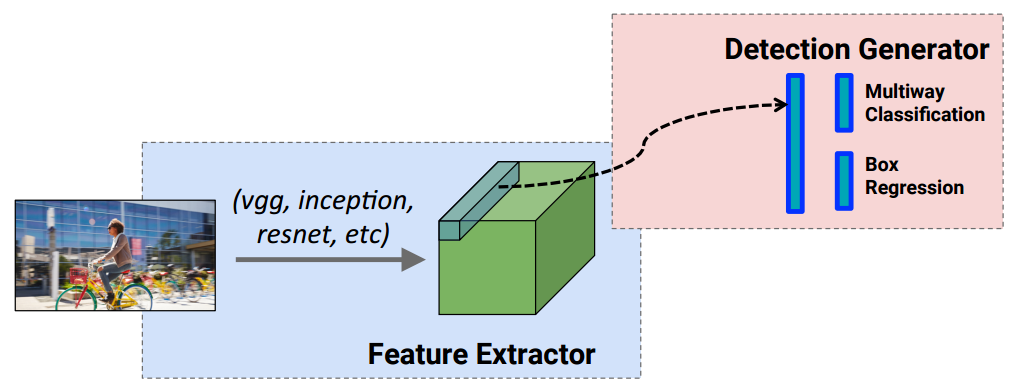
\includegraphics[width=10cm]{images/SSD_schematic}
	\caption{Schema of the SSD architecture.}
	\label{fig:perception_ssd}
\end{figure}


This network provides an accurate and efficient object detection, returning for each processed image:
\begin{itemize}
	\item \emph{Classes:} the detected classes (person, cell phone, airplane, dog \dots) inferred for each detected object.
	\item \emph{Scores:} the confidence $\in [0,1]$ the network has on each object belonging to the estimated class.
	\item \emph{Boxes:} the coordinates of the rectangular \emph{bounding box} which wraps the detected object, expressed as the coordinates of two opposite corners of it.
\end{itemize}

Although the used SSD model is capable to detect up to 80 object classes, the proposed system only retains those detection corresponding to \emph{persons}, as it is what we are interested to follow. This whole process provides a lightweight \emph{person detection}, perfectly capable to work in real time on a regular computer.

In addition, our implementation is capable to handle different network models and architectures on a \emph{plug and play} way, just pointing the model file (in the specific TensorFlow \texttt{.pb} format) in the configuration file of the program.


\subsection{Face detection}

Once the existing persons on the image have been detected, the next step is to search their faces, in order to know whether any of them corresponds to the target person to follow. In order to achieve it, the classical Viola and Jones face detection algorithm \cite{viola-jones} has been used, as it is a simple and fast solution, suitable for a prototype that already handles a \emph{SSD} CNN. This algorithm, which comprises \emph{Haar} features (Fig. \ref{fig:perception_haar}), is a simple algebraic method which takes advantage of the typical illumination pattern of a face (due to its physical shape) to detect promising regions of the input image to contain a face. To test a \emph{Haar} feature on a specific grayscale image, the feature is slided through it, and a simple operation is performed (black pixels subtracted to white ones). If the result is positive along all the feature, the region where it has been applied passes the test.


As the previous block detected persons inside the image, this face detection algorithm is only applied inside the instance of the detected persons, in order to speed up the system and avoid false positive detections. Each one of the detected persons is divided into \emph{regions}, which are passed through a \emph{cascade} of tests, where the non-compliant regions are immediately discarded. The accepted ones pass to a slightly more complex feature each time, and the regions which pass all the features are supposed to contain a face. This progressive region dismiss makes it an efficient algorithm, capable of run simultaneously with the rest of tasks. This entire process is performed with an OpenCV\footnote{Open source image processing library.} function.

\begin{figure}[h]
	\centering
	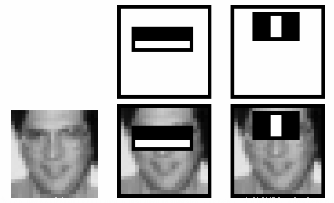
\includegraphics[width=8cm]{images/haar_on_face}
	\caption{\emph{Haar} features applied on a face.}
	\label{fig:perception_haar}
\end{figure}


\subsection{Person and face trackers}

Both previous steps detect persons and faces, but although they behave in a robust way, their outputs can suffer spurious false negative or false positive detections, due to lighting or occlusions. As they can interfere with the desired following capability, the third step palliates their effect implementing time-spatial \emph{trackers}, which filter the detection outputs (\emph{candidate detections}). The tracker associates to each person/face its coordinates inside the image, and takes into account the number of successive frames on which it has been detected. If it surpasses a \emph{patience} threshold, then it is considered a reliable (\emph{tracked}) detection. Otherwise, it is taken as a spurious output and ignored. In addition, each \emph{tracked detection} is remembered for some frames even without new updates of its current position. This way, a partial occlusion of a person does not cause her elimination, until she has not been seen for a while.
% The same happens with void detections which generally happen on a punctual way on a frame.

This tracking step can be observed in Fig. \ref{fig:perception_tracker}, in a generic \emph{instance} case (which comprises the same behavioral for person and face tracking). In addition, it is not necessary to detect the person/face every time, as the tracker is capable to infer that a new detection near the last position of a person corresponds to its new location, without requiring to see again her face to check whether she is the same person.

\begin{figure}[h]
  %	\centering
  \hspace{-0.4cm}
	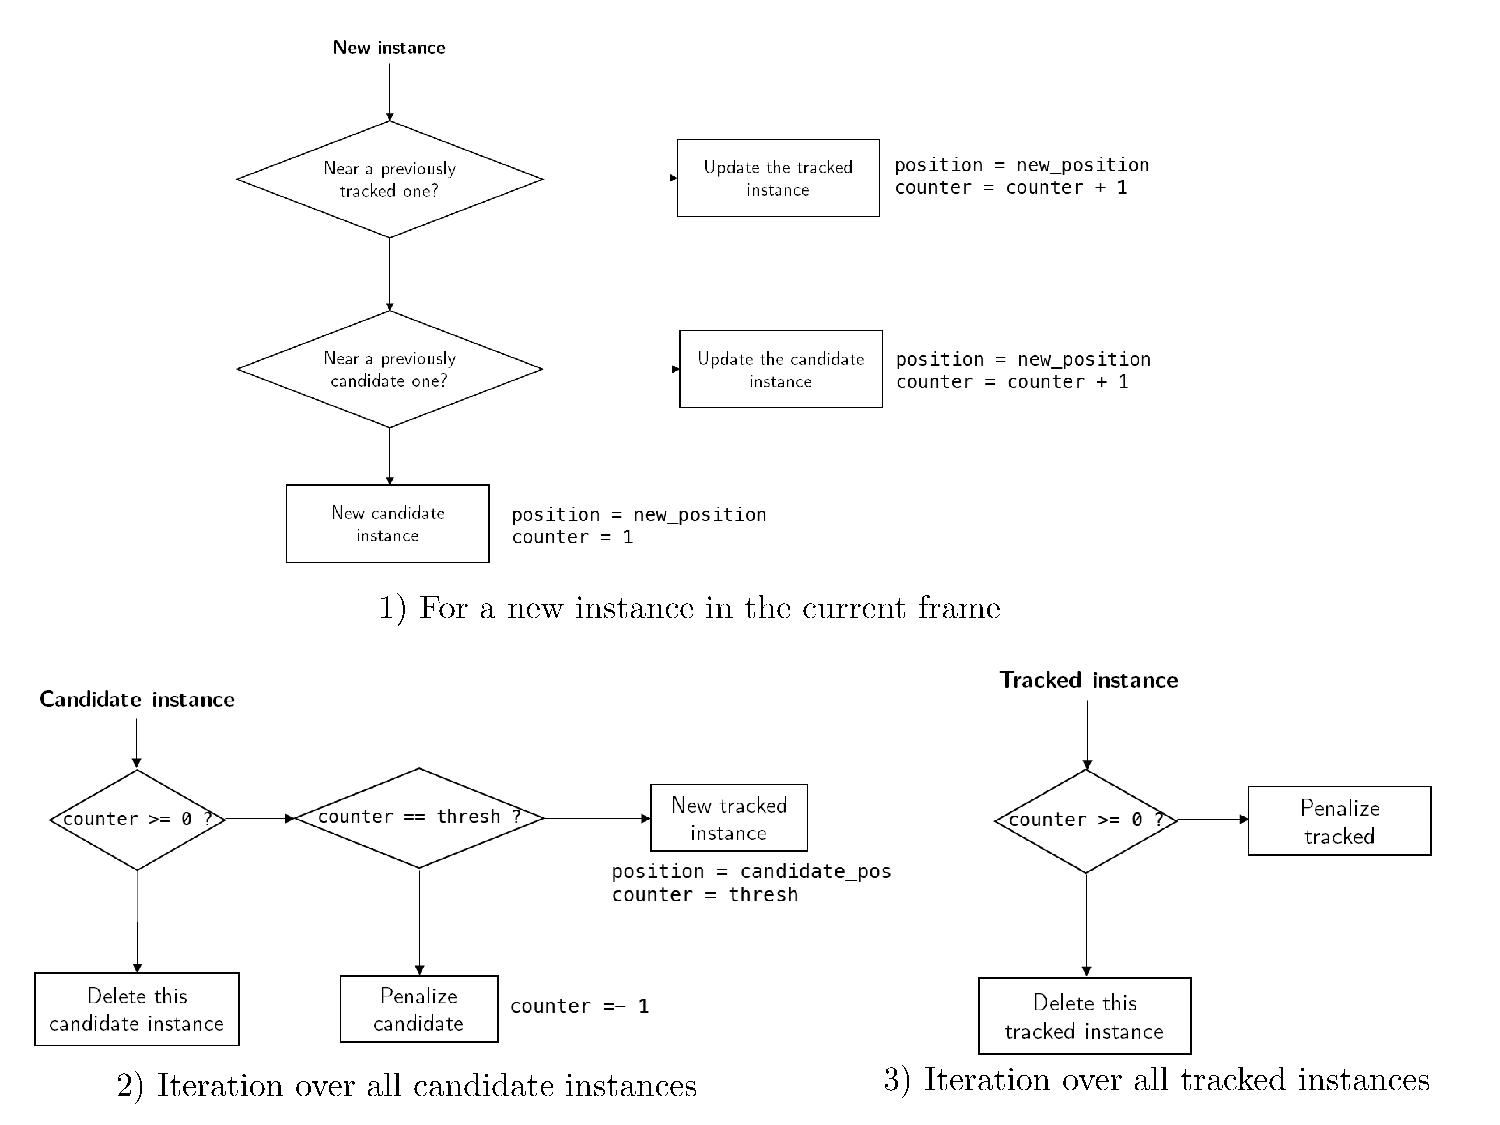
\includegraphics[width=14cm]{images/flowcharts}
	\caption{Tracking process for a instance (person/face).}
	\label{fig:perception_tracker}
\end{figure}


\subsection{Face reidentification}

The previous trackers turn the unfiltered output of the detection subsystems into tracked and more reliable detections. Hence, they can be used to perform \emph{identification} tasks. For this purpose, a parallel CNN is used, the \emph{FaceNet} \cite{facenet}. This network \emph{maps} a face image, extracting some key features, into a 128-dimensional Euclidean space, where faces are represented by what is called \emph{embeddings} (feature vectors). The Euclidean $L^2$ distance (Eq. \ref{eqn:eucl_distance}) existing between two of this embeddings stands for the \emph{face similarity} between those faces. Hence, we can consider that two embeddings belong to the same face if their distance is below a threshold, which has experimentally been set to $1.1$.

\begin{equation}
d(\vec{f_1}, \vec{f_2}) = \sqrt{\sum_{i=1}^{128}(f_{1_i} - f_{2_i})^2}
\label{eqn:eucl_distance}
\end{equation}

The proposed solution makes use of this, and computes the embeddings of each detected (and tracked) face on real time. Once this has been performed, it compares the similarity between these embeddings and the one corresponding to the target person. This target embedding is computed when the program starts, from a given image file of the \emph{person to be followed}.

To avoid penalties on similarity due to lighting conditions, a previous blurring and \emph{prewhitening} (on Eq. \ref{eqn:perception_normalization}, with $x$ as the color channel, $\mu$ as its mean and $\sigma$ as its standard deviation) are performed on each given face to the \emph{FaceNet}.

\begin{equation}
x' = \frac{x - \mu}{\sigma}
\label{eqn:perception_normalization}
\end{equation}

In Figure \ref{fig:perception_distance} the same face is seen in different lighting conditions, and all of them yield embeddings with a distance lower than the threshold.

\begin{figure}[h]
	\centering
	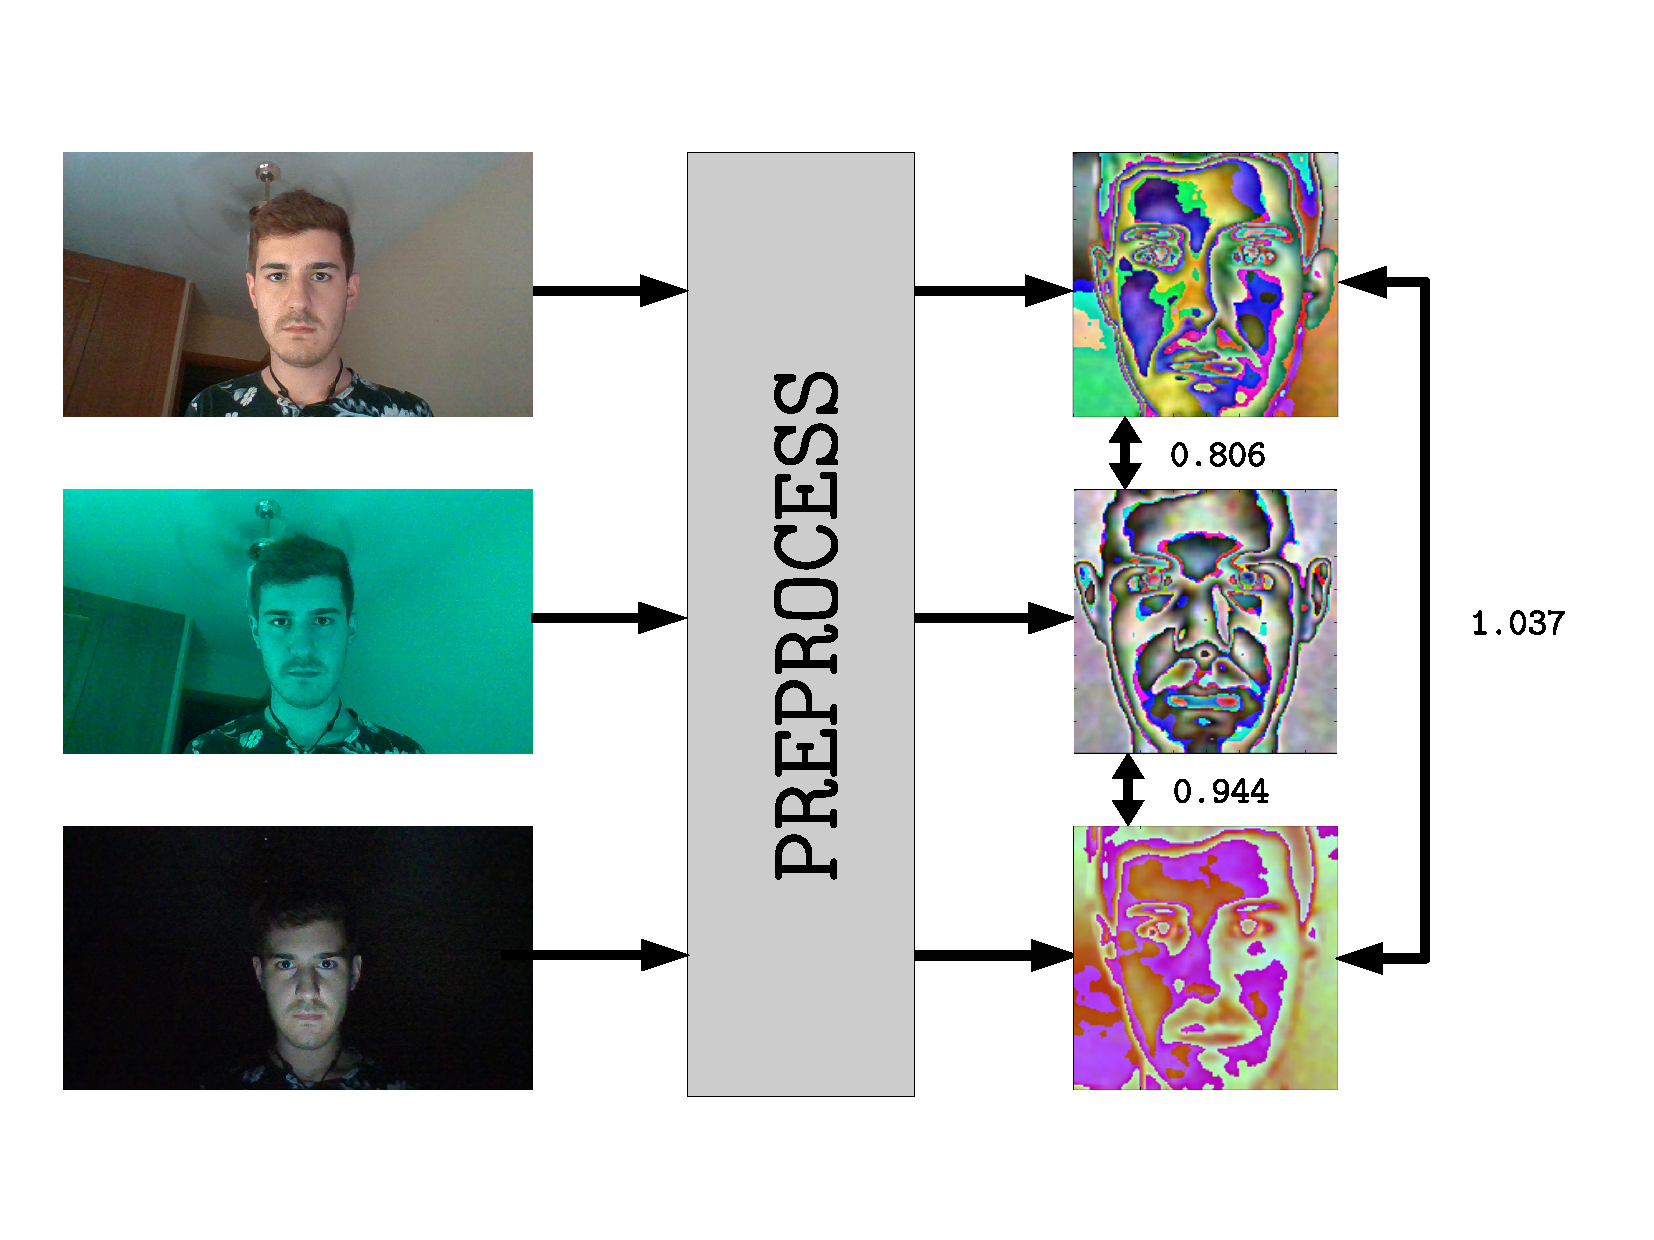
\includegraphics[width=10cm]{images/facenet_prewhiten}
	\caption{Relative distances between the same face on different lighting situations.}
        \label{fig:perception_distance}
% Color patterns on the right images are not representative, as they depend on the numeric range of the plotted image.}
\end{figure}







% ---- Actuation module ----
\section{Actuation module}

With the \emph{perception} module the system obtains the maximum possible certainty about the persons present in the current RGB image, as well as their condition of being or not the one to be followed. The \emph{actuation} module is responsible of generating a suitable command to the robot motors, in order to move towards the target person, in case it is being tracked in the current frame. To do so, it follows its own pipeline, explained next.

%\subsection{Following behavior}
% As it has been stated, 
The input for this module is the information yielded by the \emph{perception} module: the \emph{tracked persons} parameters (position, face, ``is or is not the target person"). From this information, it has to infer the proper robot movements taking also into account the state of the system on the last iteration. This is implemented with a \emph{case-based} behavior, which follows the \emph{flow chart} represented on Fig. \ref{fig:actuation_flow}. The response mainly depends on \emph{mom} (the name given to the target person), as it can be \emph{lost} or \emph{tracked and followed}.\\

\begin{figure}[h]
	\centering
	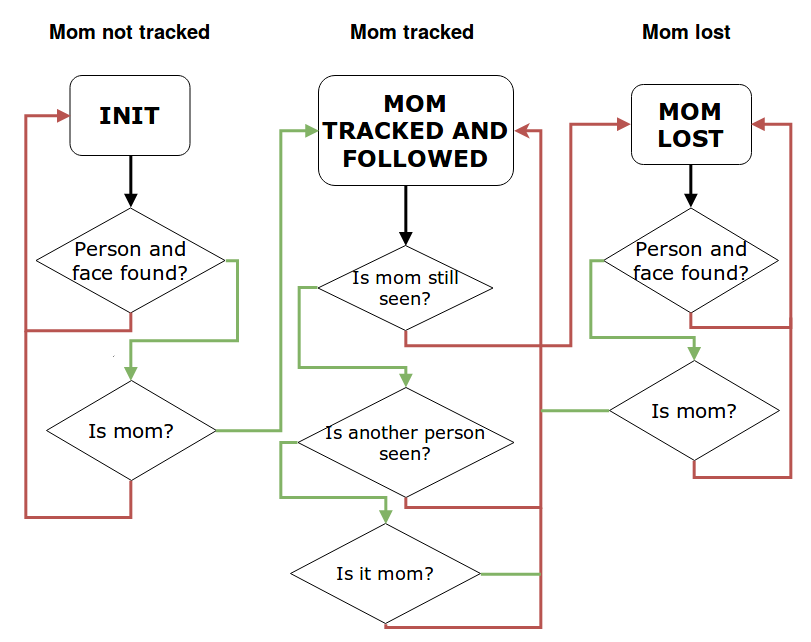
\includegraphics[width=9cm]{images/flowchart}
	\caption{\emph{Flow chart} followed by the case-based behavioral, depending on the previous state.}
	\label{fig:actuation_flow}
\end{figure}

If the target person is found among the tracked persons, the system follows it. It can be observed that the system does not need a continuous face feedback to follow the target person. The time-spatial continuity provided by the previously described trackers allows a stable tracking even when the person is only visible on its back side. In addition, if a new face is found and it satisfies the criteria of similarity with the reference face, then the \emph{followed} role is switched to that new person, which starts being followed by the robot.

This actuation module has been implemented within a computer iterative thread, and its pipeline is executed \emph{once} per thread iteration. This results on a new speed command pair (angular and linear speeds) to the motor base on each iteration.

\subsection{Error computation}

Once the system has recognized the target person inside the image, in case it is being seen, it proceeds to an \emph{error computation}, in order to determine the strength of the required rotation and traslation to move towards that person. As the robot moves over the ground plane, with two degrees of freedom, the system computes two errors: angular error and distance error.

\begin{figure}
%  \centering
  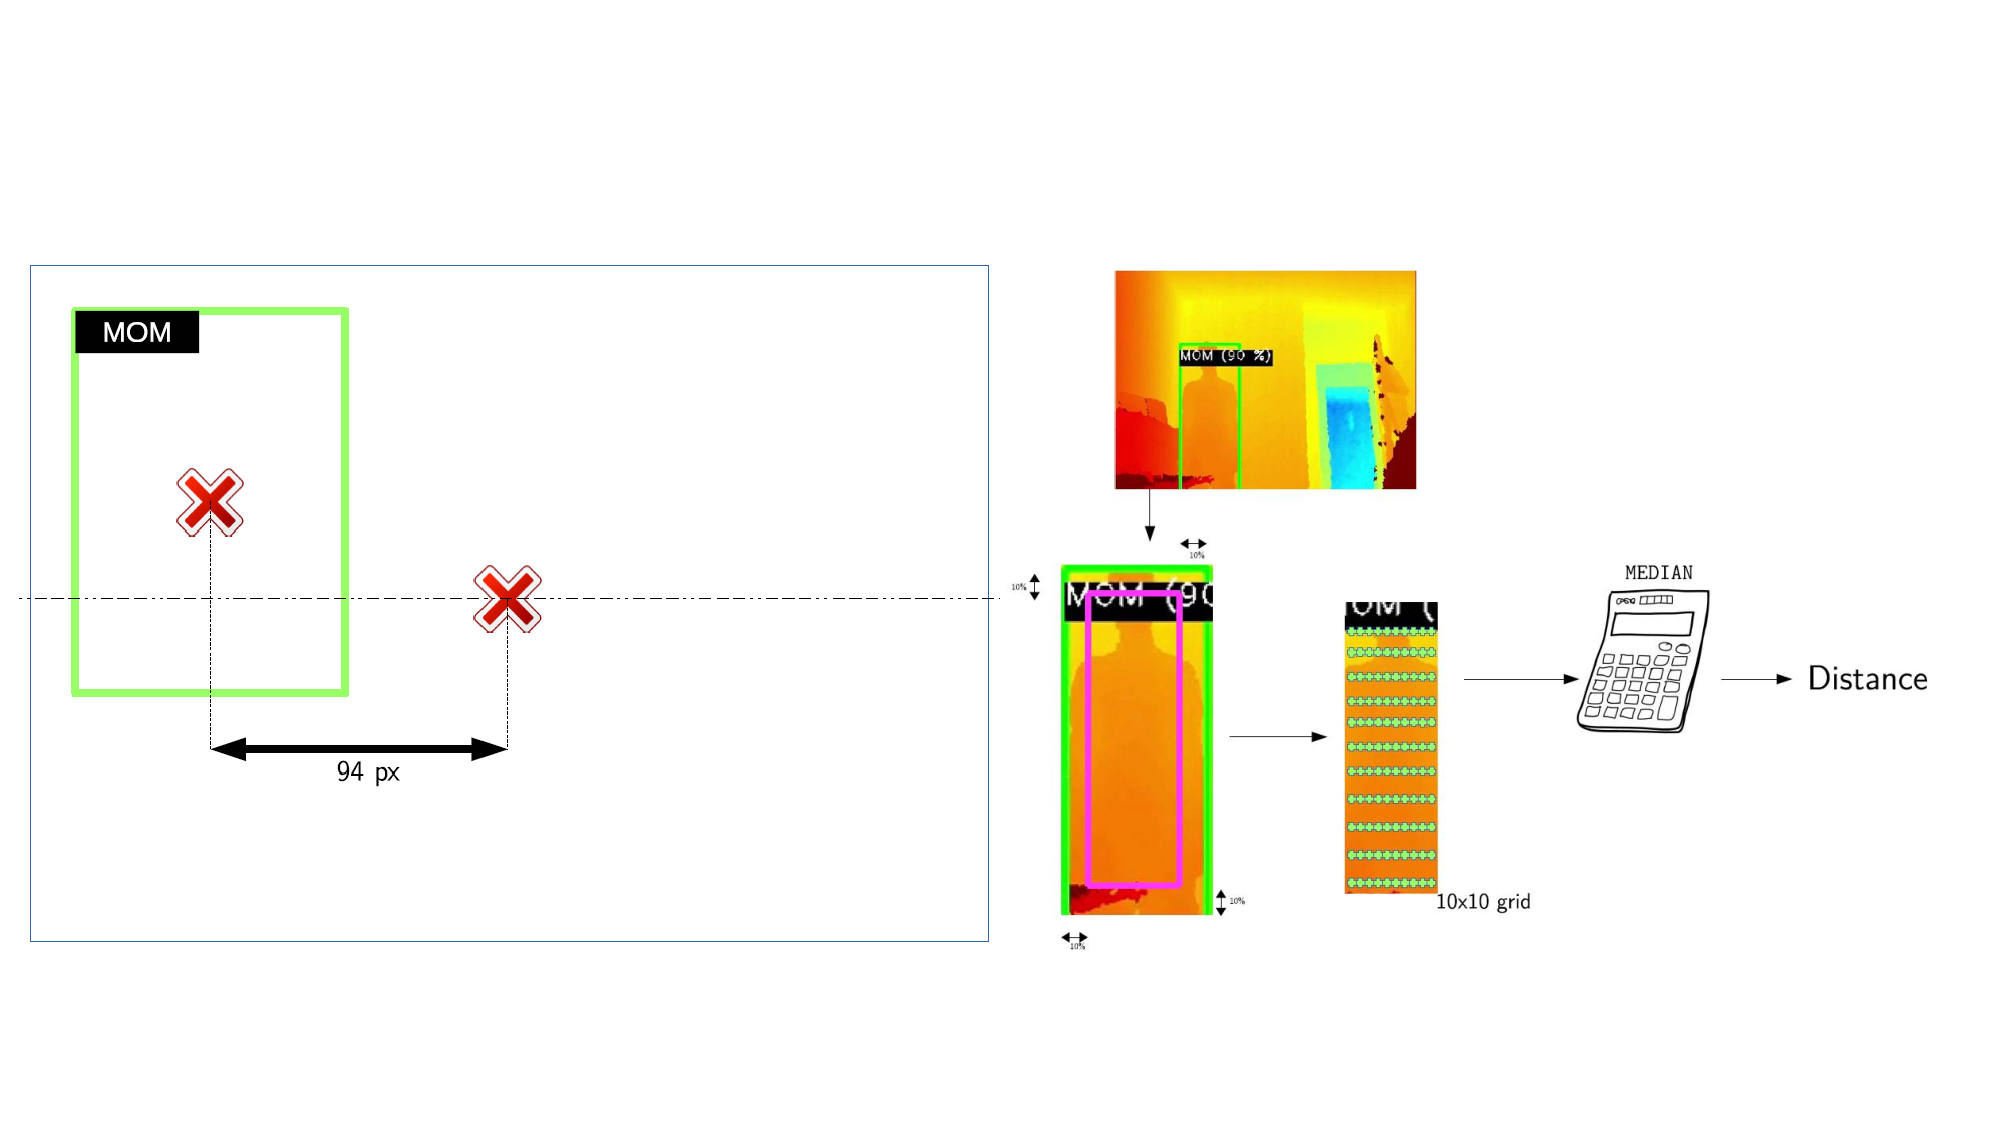
\includegraphics[width=13cm]{images/errors}
  \caption{Computation of the angular error (left) and distance error (right) between the system and the followed person.}
  \label{fig:h_error}
\end{figure}

The most desirable robot orientation with respect to the person is to be aligned with her. This way, the person appears right in the horizontal center of the image. Hence, we can compute the \emph{angular error} as the subtract of the center coordinates and the center of the person's bounding box, in the horizontal dimension (Figure \ref{fig:h_error} (left)). This error gives an approximate idea of the necessary turn to align the robot and the target person.
	
The used sensor is a RGBD camera, which provides \emph{depth} images. These depth images are aligned with the RGB ones, which means that the coordinates of the person inside the depth image are the same than the RGB ones. Hence, it allows to \emph{locate} the person inside the depth map and measure the \emph{distance error}. For the sake of robustness, this has been implemented using a 10$\times$10 grid sampling of the depth values inside the person box (putting care on avoiding the margins, in order to measure only inside the person) allows to collect a serie of measured distances to the person. It computes the \emph{median} of that set of measures, taking the result as the real distance from the robot to the person, as seen on Fig. \ref{fig:h_error} (right). 
%So far, the system is capable to determine a numerical error value to measure the magnitude of the required response.

\subsection{Movement control}

Both angular and distance errors are computed to determine the \emph{relative position} of the robot and the target person. They are used as an input to compute the most suitable control response. As the purpose is not to move the robot literally to the position of the person, but to just maintain a following behavior, a \emph{desirable zone} is established in each degree of freedom. When the target person is found inside these desirable zones (illustrated on Fig.\ref{fig:dead_zones}), the robot will not move towards her, as the person is considered \emph{under control}. They are also known as dead zones as no correction from control is needed. 

\begin{figure}[h]
	\centering
	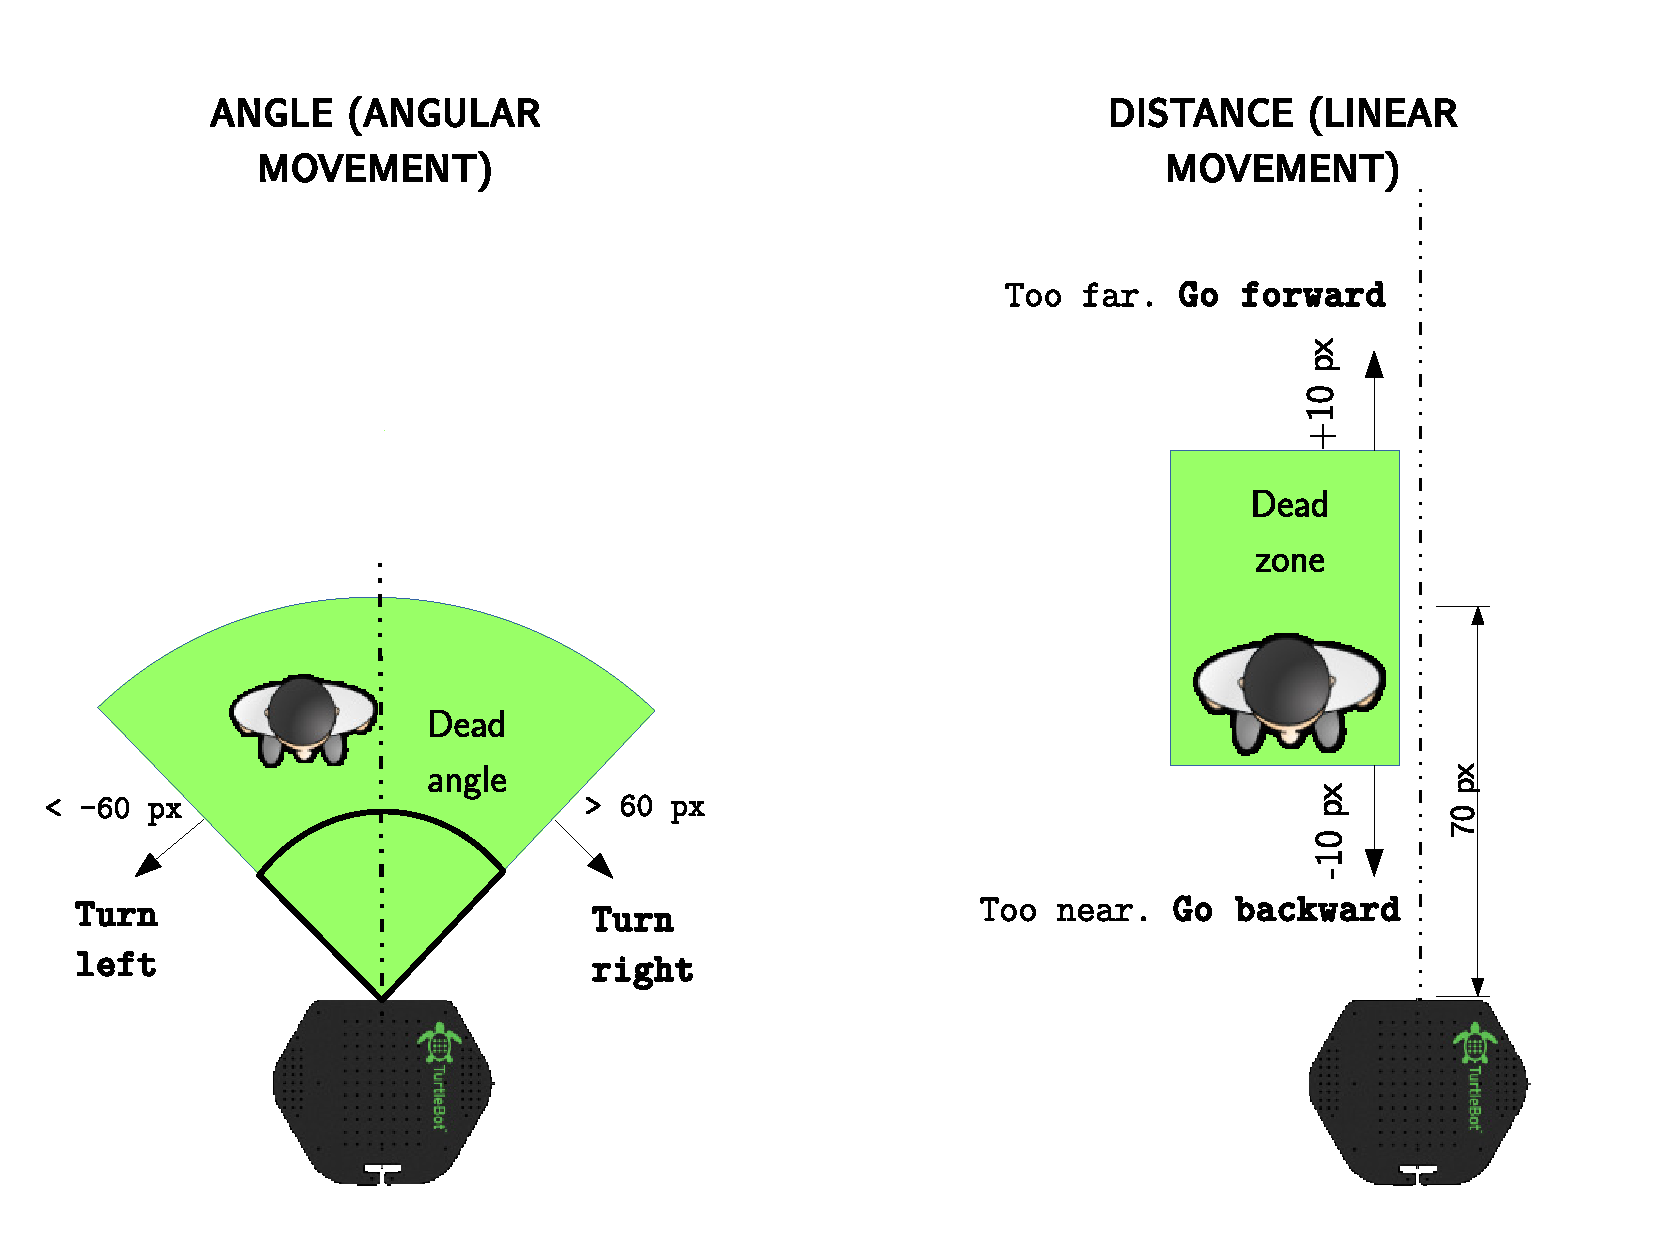
\includegraphics[width=11cm]{images/dead_zones}
	\caption{Dead zones on each dimension, where the person is considered under control.}
	\label{fig:dead_zones}
\end{figure}

If the person is outside these dead zones, a physical correction response is required, with the purpose of \emph{seeing} that person again inside the dead zone. For this action, each dimension implements a \emph{PID} controller, which establishes a \emph{closed-loop} feedback, as described on \cite{pid-controller}. This allows to keep in mind previous responses, to achieve the optimum fitting on each iteration. This means, for example, to accelerate if the person is not going any closer, or to step hard on the brake if the person suddenly gets too close.

The implemented \emph{PID} controllers (an angular and a linear one) have been experimentally tuned to obtain the most suitable parameters for our operation, obtaining the values in Table \ref{tab:pids}.

\begin{table}[h]
	\centering
	\begin{tabular}{|c|c|c|}
		\hline
		\textbf{} & \textbf{Linear} & \textbf{Angular} \\ \hline
		$k_p$     & 2               & 7                \\ \hline
		$k_d$     & 0.1             & 0.5              \\ \hline
		$k_i$     & 3               & 10               \\ \hline
	\end{tabular}
	\caption{Optimal found values for the parameters in each PID controller.}
	\label{tab:pids}
\end{table}

This way, the system can output a speed command with a tight adjustment to the values required by the situation of the current iteration. The response obtained from this value is a \emph{reactive} one. This means that each value results in a new movement command, avoiding to perform movements longer than one iteration. For softness sake, what is sent to the motors is not that value, but the \emph{mean} between it and the last sent one. This way, it results on a slightly longer convergence that helps to remove sudden movements.




% ---- Experiments ----
\section{Experiments}
\label{sec:experiments}

This entire approach has been experimentally validated on a real system\footnote{Full video test available on \url{https://www.youtube.com/watch?v=oKMR_QCT7EE}}, composed by:

\begin{itemize}
	\item Asus Xtion Pro Live RGBD sensor.
	\item Turtlebot2 robot.
	\item Standard laptop computer. Hardware:
	\begin{itemize}
		\item CPU: Intel i5-4210U
		\item RAM: 8 GB DDR3L
		\item GPU: Nvidia 940M
	\end{itemize}
\end{itemize}

\begin{figure}[h]
	\centering
	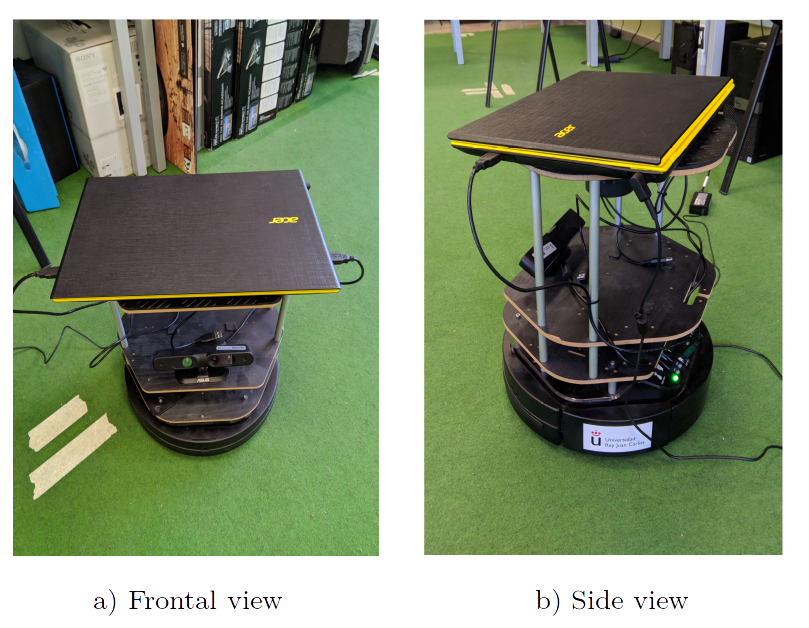
\includegraphics[width=4in]{images/exp_set}
	\caption{Experimental set where the system has been validated.}
	\label{fig:exp_set}
\end{figure}






The results have yielded a fine following system, which only follows to the indicated person, with a refresh rate of 10 movements per second (as the SSD CNN is the lightest possible model, as seen on Table \ref{tab:model_tests}. This helped substantially to minimize the time bottleneck). The tracking and reidentification process can be observed on the highest region of Fig. \ref{fig:exp_figures}. The following process can be observed on the lowest region of Fig. \ref{fig:exp_figures}.

\begin{figure}[h]
	\centering
	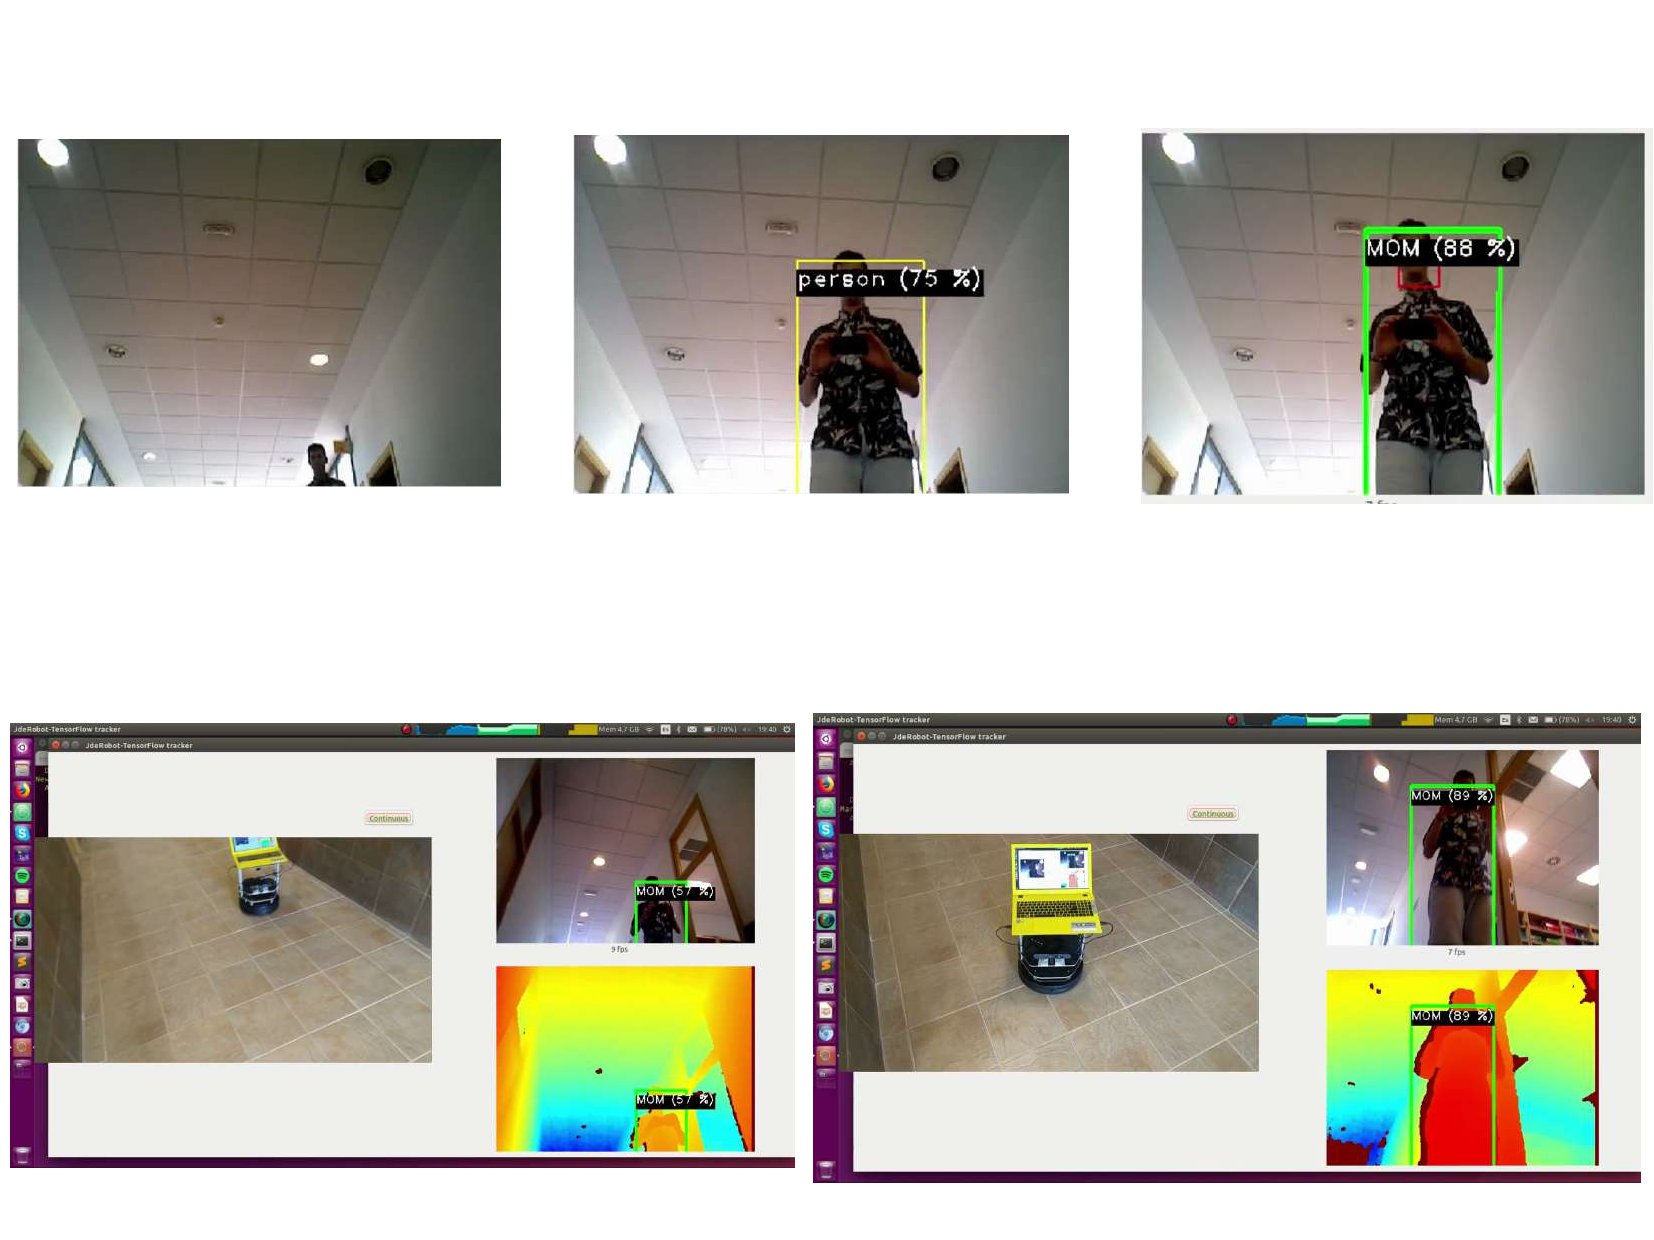
\includegraphics[width=2.5in]{images/exp_figures}
	\caption{Tracking and reidentification process for a person (up). Following process (down).}
	\label{fig:exp_figures}
\end{figure}

% ---- Conclusions ----
\chapter{Conclusions}
\section{Conclusions}
	This final chapter will be devoted to revisit the  proposed objectives. They could be summarized in a central purpose: \emph{enriching the JdeRobot framework with new tools and applications focused on deep learning}. With a complete coverage of the performed tasks, as it has been described on the previous pages, we can contrast what has been achieved on each milestone which was established along the way, in order to accomplish incremental achievements.\\
	
	\begin{description}
		\item[Classification tool for processing live images.] \hfill
			\vspace{0.2in} \\
			The first objective was to upgrade the scope for an existing JdeRobot tool, \texttt{DigitClassifier}, which was designed to perform \emph{classification} tasks using \emph{deep learning} techniques.\\
			
			Its functionality was extended to support the \emph{deep learning} framework TensorFlow, implementing and training networks on our own. This has allowed to achieve initial knowledge about the framework, and enough skills to move towards more complex tasks.\\
			
			In light of the excellent achieved performance, the brand new TensorFlow implementation and the previous one (made with the Keras framework) were merged into an \emph{official JdeRobot} component\footnote{\url{https://github.com/JdeRobot/dl-digitclassifier}}, capable of commuting between both frameworks.
		
		\item[Neural detection tool for live images.] \hfill
			\vspace{0.2in} \\		
			After having accomplished a basic domain on \emph{deep learning} with \emph{classification} tasks, we tackled a more ambitious milestone: \emph{detecting objects on a real-time operation}. There was no previous reference in the JdeRobot framework.\\
			
			The process of training a detection network was ruled out of the scope of this project, so we addressed the detection task using publicly available \emph{pretrained networks}. So, we developed a wrapping of TensorFlow environment to \emph{abstract} the model (architecture, dataset on which it was trained, output format, etc.), and moved the neural network processing to a \emph{GPU environment} (to achieve the optimum predicting rate for a real-time operation). This remarkably efficient detection framework was demonstrated to be capable of real-time processing, so we have developed an entire node, \texttt{ObjectDetector}, to visually perform this task on an \emph{incoming image stream} (abstracting the source).\\
			
			Hence, the final result  has been a node displaying the raw current image, and aside the same one with the detected objects overlaid, indicating their location making use of \emph{bounding boxes}, in addition to the estimated \emph{class} for the object, and the \emph{score} (standing for the reliability level that estimation has).\\
			
			Once more, the excellent performance on real-time (using detectors with a SSD architecture for instance) has driven us to integrate this node\footnote{\url{https://github.com/JdeRobot/dl-objectdetector}} in the JdeRobot framework as well, developing another module to do the same for Keras network models. This has enabled us again to be able to abstract the frameworks, and toggle one of them through the YML file. In addition, this has given us the capability of \emph{benchmarking} new models, as they can be transparently loaded into the created environment, and begin making inferences on real time.
		
		\item[Tracking and following robot behavior using deep learning detection] \hfill
			\vspace{0.2in} \\
			The two previous milestones allowed us to accomplish \emph{state-of-the-art} purposes in the \emph{Computer Vision} field. As the final research objective, we have considered an \emph{actuation} system which uses a powerful \emph{neural network} to accomplish an robust visual perception. In order to overlap our research with the prosperous field of \emph{robotics}, we have developed a component capable of \emph{following} a specific person (\emph{mom}). This has been achieved using concepts like a \emph{PID} controller feedback control, and case-based control.\\
			
	\end{description}
	
	All these achievements have contributed the JdeRobot framework with an upgraded tool (\emph{DigitClassifier}, which now offers support for both Keras and TensorFlow), a brand new tool (\emph{ObjectDetector}), and a new robotics application (\emph{FollowPerson}, capable of chasing a person with excellent results). These new resources are focused on providing real time operation. In addition, all the underlying software created (the \emph{TensorFlow} and \emph{Keras} generic network loaders) can be of great help for future applications.\\
	
	Beyond the technical contents, this project has allowed an interested person in \emph{deep learning} to learn about a cornucopia of concepts and experience. A while ago, when it was decided to evolve towards creating a reactive behavioral, it was motivating to make the most of a possible synergy between two different fields of knowledge, as \emph{deep learning} and \emph{robotics} are.\\
	
	In the professional point of view, it has been essential to acquire further skills about \emph{version control systems}, as Git. This can be an important benefit, as every development project in a corporate environment makes use of this kind of controls.

\section{Future lines}
	The proposed milestones on this project have been successfully achieved using a useful and innovative tool as \emph{deep learning}. Furthermore, it opens some interesting doors to future research or improvements:
	
	\begin{itemize}
		\item \emph{Upgrade DigitClassifier:} for now, this component looks for the digit in a fixed window inside the input image (the central square). Another module could be implemented to perform a \emph{character detection} in the whole image, maybe an OCR number detector.
		
		\item \emph{Translate the Python nodes to a compiled and fast language:} one of the main handicaps of Python is the fact that it is an interpreted language (much slower than a compiled one). So, a \emph{translation} to a lower level language as \texttt{C++} would be very interesting, as it is a widely supported language in this framework, and there are already very efficient \emph{deep learning} implementations on it (as \emph{Darknet/YOLO}).
		
		\item \emph{Use a deep learning face detector in FollowPerson:} the main advantage of the \emph{deep learning} systems is the robustness on their operation, so a facial detection system implemented with this technology could be a powerful resource to perform a facial detection/validation in harshly lightened environments.
		
		\item \emph{Multimodal person detection/tracking:} some extra functionality could be squeezed from a RGBD sensor, like \emph{tracking a person in complete darkness}. As \emph{deep learning} systems offer good results distinguishing a person silhouette, we could perform people detection on a depth image.
		
		
		\item \emph{Add a navigation algorithm to FollowPerson:} the movement commands sent to the Turtlebot are now decided taking into account only the relative position of the person from the robot. However, as the robot incorporates a laser sensor, we can add an \emph{obstacle avoidance} system, in order to perform a non-blind navigation towards the person.
	\end{itemize}









% ---- Bibliography ----
%
\begin{thebibliography}{6}
  %

\bibitem{dalal2005}
Dalal, Navneet and Triggs, Bill.
Histograms of oriented gradients for human detection, 
IEEE Computer Society Conference on Computer Vision and Pattern Recognition, 2005. CVPR 2005.
%  volume={1},
%  pages={886--893},

\bibitem{munoz2007people}
Mu{\~n}oz-Salinas, Rafael and Aguirre, Eugenio and Garc{\'\i}a-Silvente, Miguel.
People detection and tracking using stereo vision and color
\textit{Image and Vision Computing} 25(6), Elsevier, 2007.
% @article{munoz2007people,
%   title={People detection and tracking using stereo vision and color},
%   author={Mu{\~n}oz-Salinas, Rafael and Aguirre, Eugenio and Garc{\'\i}a-Silvente, Miguel},
%   journal={Image and Vision Computing},
%   volume={25},
%   number={6},
%   pages={995--1007},
%   year={2007},
%   publisher={Elsevier}
% }

% \bibitem{aguirre2014leg}
% Aguirre, Eugenio and Garcia-Silvente, Miguel and Plata, Javier.
% Leg detection and tracking for a mobile robot and based on a laser device, supervised learning and particle filtering
% \textit{ROBOT2013: First Iberian Robotics Conference}, Springer, 2014.
% @inproceedings{aguirre2014leg,
%   title={Leg detection and tracking for a mobile robot and based on a laser device, supervised learning and particle filtering},
%   author={Aguirre, Eugenio and Garcia-Silvente, Miguel and Plata, Javier},
%   booktitle={ROBOT2013: First Iberian Robotics Conference},
%   pages={433--440},
%   year={2014},
%   organization={Springer}
% }

\bibitem{aguirre2016multisensor}
Aguirre, Eugenio and Garc{\'\i}a-Silvente, Miguel and Pascual, Daniel,
A multisensor based approach using supervised learning and particle filtering for people detection and tracking,
\textit{Robot 2015: Second Iberian Robotics Conference}, Springer, 2016
% @inproceedings{aguirre2016multisensor,
%   title={A multisensor based approach using supervised learning and particle filtering for people detection and tracking},
%   author={Aguirre, Eugenio and Garc{\'\i}a-Silvente, Miguel and Pascual, Daniel},
%   booktitle={Robot 2015: Second Iberian Robotics Conference},
%   pages={645--657},
%   year={2016},
%   organization={Springer}
% }

\bibitem {rocapal2005}
%Calvo, R.: Comportamiento sigue persona con visión direccional, Proyecto Fin de Carrera, Universidad Rey Juan Carlos, 2004.
R.Calvo, J.M.Cañas, L.García-Pérez. 
Person following behavior generated with JDE schema hierarchy 
\textit{Poster in ICINCO 2nd Int. Conf. on Informatics in Control, Automation and Robotics}. Barcelona (Spain), sep 14-17, 2005. INSTICC Press, pp 463-466, 2005. ISBN: 972-8865-30-9

\bibitem {ssd}
Lui, W., Anguelov, D., Erhan, D., et al. 
SSD: Single-Shot Multibox Detector. 
\emph{CoRR}, abs/1512.02325, 2015.

\bibitem {viola-jones}
Viola, P., Jones, M. 
Rapid object detection using a boosted cascade of simple features. 
In \emph{Proceedings of the 2001 IEEE Computer Society Conference on Computer Vision and Pattern Recognition. CVPR 2001}, volume 1, pages I-511-I-518 vol.1, 2001.

\bibitem{facenet}
Schroff, F., Kalenichenko, D., Philbin, J. 
\emph{FaceNet}: A unified embedding for face recognition and clustering. 
\emph{CoRR}, abs/1503.038032, 2015.

\bibitem{pid-controller}
Åström, KJ., Murray, RM. 
\textit{Feedback Systems: An Introduction for Scientists and Engineers}, 2004.

\bibitem{xue2016tracking}
Xue, Hongyang and Liu, Yao and Cai, Deng and He, Xiaofei. 
Tracking people in RGBD videos using deep learning and motion clues. 
\textit{Neurocomputing} 204, pages 70-76, Elsevier, 2016. 
% @article{xue2016tracking,
%   title={Tracking people in RGBD videos using deep learning and motion clues},
%   author={Xue, Hongyang and Liu, Yao and Cai, Deng and He, Xiaofei},
%   journal={Neurocomputing},
%   volume={204},
%   pages={70--76},
%   year={2016},
%   publisher={Elsevier}
% }

\bibitem{koide2016identification}
Koide, Kenji and Miura, Jun.
Identification of a specific person using color, height, and gait features for a person following robot.
\textit{Robotics and Autonomous Systems} 84, pages 76-87, Elsevier, 2016.
% @article{koide2016identification,
%   title={Identification of a specific person using color, height, and gait features for a person following robot},
%   author={Koide, Kenji and Miura, Jun},
%   journal={Robotics and Autonomous Systems},
%   volume={84},
%   pages={76--87},
%   year={2016},
%   publisher={Elsevier}
% }

\bibitem{munaro2014feature}
Munaro, Matteo and Ghidoni, Stefano and Dizmen, Deniz Tartaro and Menegatti, Emanuele.
\textit{A feature-based approach to people re-identification using skeleton keypoints}.
2014 IEEE International Conference on Robotics and Automation (ICRA). 
% @inproceedings{munaro2014feature,
%   title={A feature-based approach to people re-identification using skeleton keypoints},
%   author={Munaro, Matteo and Ghidoni, Stefano and Dizmen, Deniz Tartaro and Menegatti, Emanuele},
%   booktitle={Robotics and Automation (ICRA), 2014 IEEE International Conference on},
%   pages={5644--5651},
%   year={2014},
%   organization={IEEE}
% }


\bibitem{welsh2017real}
Welsh, John Bradford.
Real-Time Pose Based Human Detection and Re-identification with a Single Camera for Robot Person Following.
\textit{PhD Thesis, University of Maryland, College Park}, 2017.
% @phdthesis{welsh2017real,
%   title={Real-Time Pose Based Human Detection and Re-identification with a Single Camera for Robot Person Following},
%   author={Welsh, John Bradford},
%   year={2017},
%   school={University of Maryland, College Park}
% }

\bibitem{yoon2016person}
Yoon, Y and Yoon, H and Kim, J
Person Reidentification in a Person-following Robot
25th \textit{IEEE International Symposium on Robot and Human Interactive Communication (RO-MAN)}, 2016.
% @Inproceedings{yoon2016person,
%   title={Person Reidentification in a Person-following Robot},
%   author={Yoon, Y and Yoon, H and Kim, J},
%   booktitle={25th IEEE International Symposium on Robot and Human Interactive Communication (RO-MAN)},
%   year={2016}
% }

\bibitem{shimura2014research}
Shimura, Kouyou and Ando, Yoshinobu and Yoshimi, Takashi and Mizukawa, Makoto. 
Research on person following system based on RGB-D features by autonomous robot with multi-kinect sensor.
2014 \textit{IEEE/SICE International Symposium on System Integration (SII)}.
% @inproceedings{shimura2014research,
%   title={Research on person following system based on RGB-D features by autonomous robot with multi-kinect sensor},
%   author={Shimura, Kouyou and Ando, Yoshinobu and Yoshimi, Takashi and Mizukawa, Makoto},
%   booktitle={System Integration (SII), 2014 IEEE/SICE International Symposium on},
%   pages={304--309},
%   year={2014},
%   organization={IEEE}
% }

\bibitem{ilias2014nurse}
Ilias, B and Shukor, SA Abdul and Yaacob, S and Adom, AH and Razali, MH Mohd.
A nurse following robot with high speed Kinect sensor.
\textit{ARPN Journal of Engineering and Applied Sciences} 9(12), pages 2454-2459, 2014.
% @article{ilias2014nurse,
%   title={A nurse following robot with high speed Kinect sensor},
%   author={Ilias, B and Shukor, SA Abdul and Yaacob, S and Adom, AH and Razali, MH Mohd},
%   journal={ARPN Journal of Engineering and Applied Sciences},
%   volume={9},
%   number={12},
%   pages={2454--2459},
%   year={2014}
% }

\bibitem{yoshimi2006development}
Yoshimi, Takashi and Nishiyama, Manabu and Sonoura, Takafumi and Nakamoto, Hideichi and Tokura, Seiji and Sato, Hirokazu and Ozaki, Fumio and Matsuhira, Nobuto and Mizoguchi, Hiroshi.
Development of a person following robot with vision based target detection.
2006 \textit{IEEE/RSJ International Conference on Intelligent Robots and Systems}.
% @inproceedings{yoshimi2006development,
%   title={Development of a person following robot with vision based target detection},
%   author={Yoshimi, Takashi and Nishiyama, Manabu and Sonoura, Takafumi and Nakamoto, Hideichi and Tokura, Seiji and Sato, Hirokazu and Ozaki, Fumio and Matsuhira, Nobuto and Mizoguchi, Hiroshi},
%   booktitle={Intelligent Robots and Systems, 2006 IEEE/RSJ International Conference on},
%   pages={5286--5291},
%   year={2006},
%   organization={IEEE}
% }

\bibitem{satake2009robust}
Satake, Junji and Miura, Jun.
Robust stereo-based person detection and tracking for a person following robot.
\textit{ICRA Workshop on People Detection and Tracking}, 2009.
% @inproceedings{satake2009robust,
%   title={Robust stereo-based person detection and tracking for a person following robot},
%   author={Satake, Junji and Miura, Jun},
%   booktitle={ICRA Workshop on People Detection and Tracking},
%   pages={1--10},
%   year={2009}
% }


\bibitem{sidenbladh1999person}
Sidenbladh, Hedvig and Kragic, Danica and Christensen, Henrik I.
A person following behaviour for a mobile robot
\textit{Proceedings of the IEEE International Conference on Robotics and Automation}, 1999. 
% @inproceedings{sidenbladh1999person,
%   title={A person following behaviour for a mobile robot},
%   author={Sidenbladh, Hedvig and Kragic, Danica and Christensen, Henrik I},
%   booktitle={Robotics and Automation, 1999. Proceedings. 1999 IEEE International Conference on},
%   volume={1},
%   pages={670--675},
%   year={1999},
%   organization={IEEE}
% }

\bibitem{mobilenet}
Howard, Andrew G. and Monglong Zhu et al.
MobileNets: Efficient Convolutional Neural Networks for Mobile Vision
\textit{CoRR journal}, volume 1704.04861, 2017.
%@article{DBLP:journals/corr/HowardZCKWWAA17,
%	author    = {Andrew G. Howard and
%		Menglong Zhu and
%		Bo Chen and
%		Dmitry Kalenichenko and
%		Weijun Wang and
%		Tobias Weyand and
%		Marco Andreetto and
%		Hartwig Adam},
%	title     = {MobileNets: Efficient Convolutional Neural Networks for Mobile Vision
%		Applications},
%	journal   = {CoRR},
%	volume    = {abs/1704.04861},
%	year      = {2017},
%	url       = {http://arxiv.org/abs/1704.04861},
%	archivePrefix = {arXiv},
%	eprint    = {1704.04861},
%	timestamp = {Mon, 13 Aug 2018 16:46:35 +0200},
%	biburl    = {https://dblp.org/rec/bib/journals/corr/HowardZCKWWAA17},
%	bibsource = {dblp computer science bibliography, https://dblp.org}
%}

\end{thebibliography}
\end{document}
